\section{Numerical implementations using standard finite elements}
\label{sec:micromorphicdamage:test_cases}

In this section, the proposed micromorphic apporoach to brittle fracture
is evaluated on numerical applications.
% classical test cases taken from the literature.
The first three are classical test cases taken from the literature and have been performed using the
\texttt{mgis.fenics} implementation. Implementations are freely available on the following repository: \url{https://github.com/davidsiedel/micromorphic-damagc-giens-2022}.
They aim at comparing both the classical phase field approach to the proposed micromorphic one.
The last two test cases are performed using the \texttt{mfem.fenics} implementation, and showcase respectively
the performance of the micromorphic approach with high order finite
elements in the case of shear driven fracture, and the scalability of the approach.

\paragraph{Hypotheses}

For the first two and the last applications in this section, a spectral decomposition of the thermo-elastic energy potential
$\psi_{\tensoriis{\varepsilon}}$ in the framework of
small deformations is considered, where $\tensorii{\varepsilon}$ denotes the linearized strain tensor.
Test cases in 2 dimension assume a plane strain hypothesis.
% , and the framework of
% small deformations is adopted.
The penalization parameter $H_{\chi}$ is chosen as
%
%
%
\begin{equation}
  H_{\chi} = \beta\,\Frac{G_{c}}{\ell_{c}}
\end{equation}
%
%
%
where $\beta$ is a normalized penalization parameter \cite{bharali_computational_2021}.

\paragraph{Choice of the convergence criterion of the staggered schemes}

In this paper, the staggered schemes are stopped when the damage becomes
stationnary, i.e. when the absolute difference between two estimates of
the damge is below a given threshold \(\varepsilon_{d}\) at each
integration point.
%
%
%
This criterion is not totally satisfying as it does not ensure that a
true minimum of the Lagrangian is found. Therefore, this second criterion has been carefully checked
for each steps of the numerical experiments described in
this section.

% \subsection{Comparison of the micromorphic solutions to the phase-field solutions on selected test cases  using \texttt{mgis.fenics}}

\subsection{Tensile test on a fiber reinforced matrix}

% The first test case of the following benchmark is taken from 

% ---------------------------------------------------------
% PARAGRAPH
% ---------------------------------------------------------
\paragraph{Specimen and loading}

The considered test case taken from \cite{bourdin_numerical_2000} describes a matrix represented by a square of length 1mm,
that is attached to a fiber in the middle (see Figure \ref{fig:micromorphic_formulation:matrix_fiber}).
The fiber is depicted by a hole
of radius 0.2mm located at the center of the specimen, and is considered to be infinitely stiff with
respect to the matrix.
A vertical displacement of amplitude 0.125mm is applied at the top of the specimen, and the
matrix is clamped around the fiber in both directions.
Damage is enforced to be null at the intersection between the matrix and the fiber, and natural
boundary conditions are considered elsewhere.

\begin{figure}[H]
    \centering
    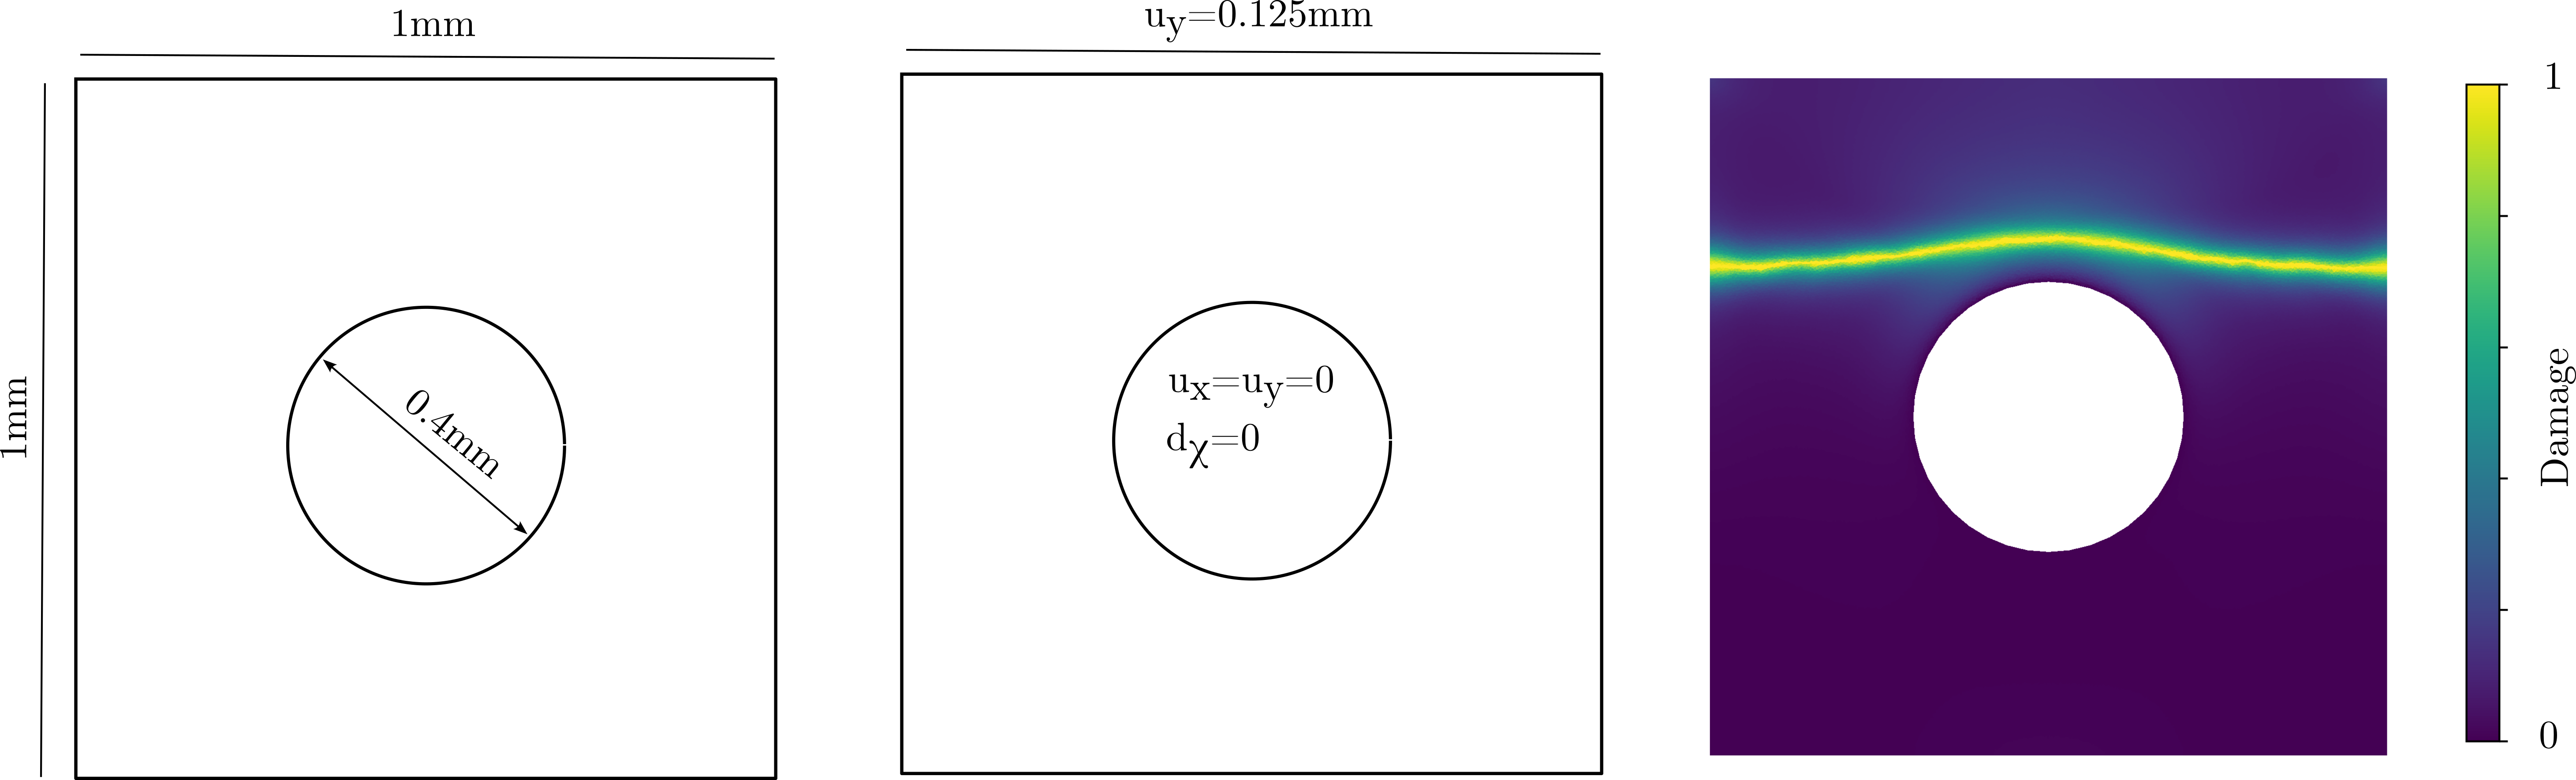
\includegraphics[width=14.cm]{../chapter_003_ef_micromorphic/drawings/matrix_mesh.png}
    \caption{Geometry, boundary conditions and damage pattern}
    \label{fig:micromorphic_formulation:matrix_fiber}
\end{figure}

% ---------------------------------------------------------
% PARAGRAPH
% ---------------------------------------------------------
\paragraph{Material behaviour}

A linear thermo-elastic energy potential $\psi_{\tensoriis{\varepsilon}}$ is considered,
with a Young's modulus $E$ equal to $200$ MPa. The material displays a compressible
behaviour with a Poisson's ratio $\nu$ equal to $0.2$.
The chosen micromorphic model is that corresponding to a AT2 model, and is described by Equations \eqref{eq:ef_micromorphic:formulation:AT2_link},
where the fracture energy release rate $G_c$ is equal to $1$ J/mm${}^2$, and the characteristic length is $\ell_c = 0.02$ mm.
Moreover, the degradation function acts on the spherical part of free energy potential (See Section \ref{sec:micromorphic:deviatori_split})
% The penalization factor $\beta$ has been tests with several values.

\paragraph{Force delfection curve}

Figure \ref{fig:micromorphic_damage:force} displays the force-deflection curves
for the tensile test on a fiber reinforced matrix, using either the proposed micromorphic
approach, an AT2 phase field approach based on the resolution of the Karush–Kuhn–Tucker conditions
to enforce irreversibility of the damage field, or an AT2 phase field approach based on the definition
of Miehe's history function \cite{miehe_phase_2010}.
The third resolution scheme depicted in Section \ref{sec:micromorphic:third_scheme} is considered for the
micromorphic approach.
As illustrated by Figure \ref{fig:micromorphic_damage:force}, the
force-displacement curve of the third scheme is very similar to the
standard AT2 model based on the resolution of the variational inequality.

\begin{figure}[H]
  \centering
  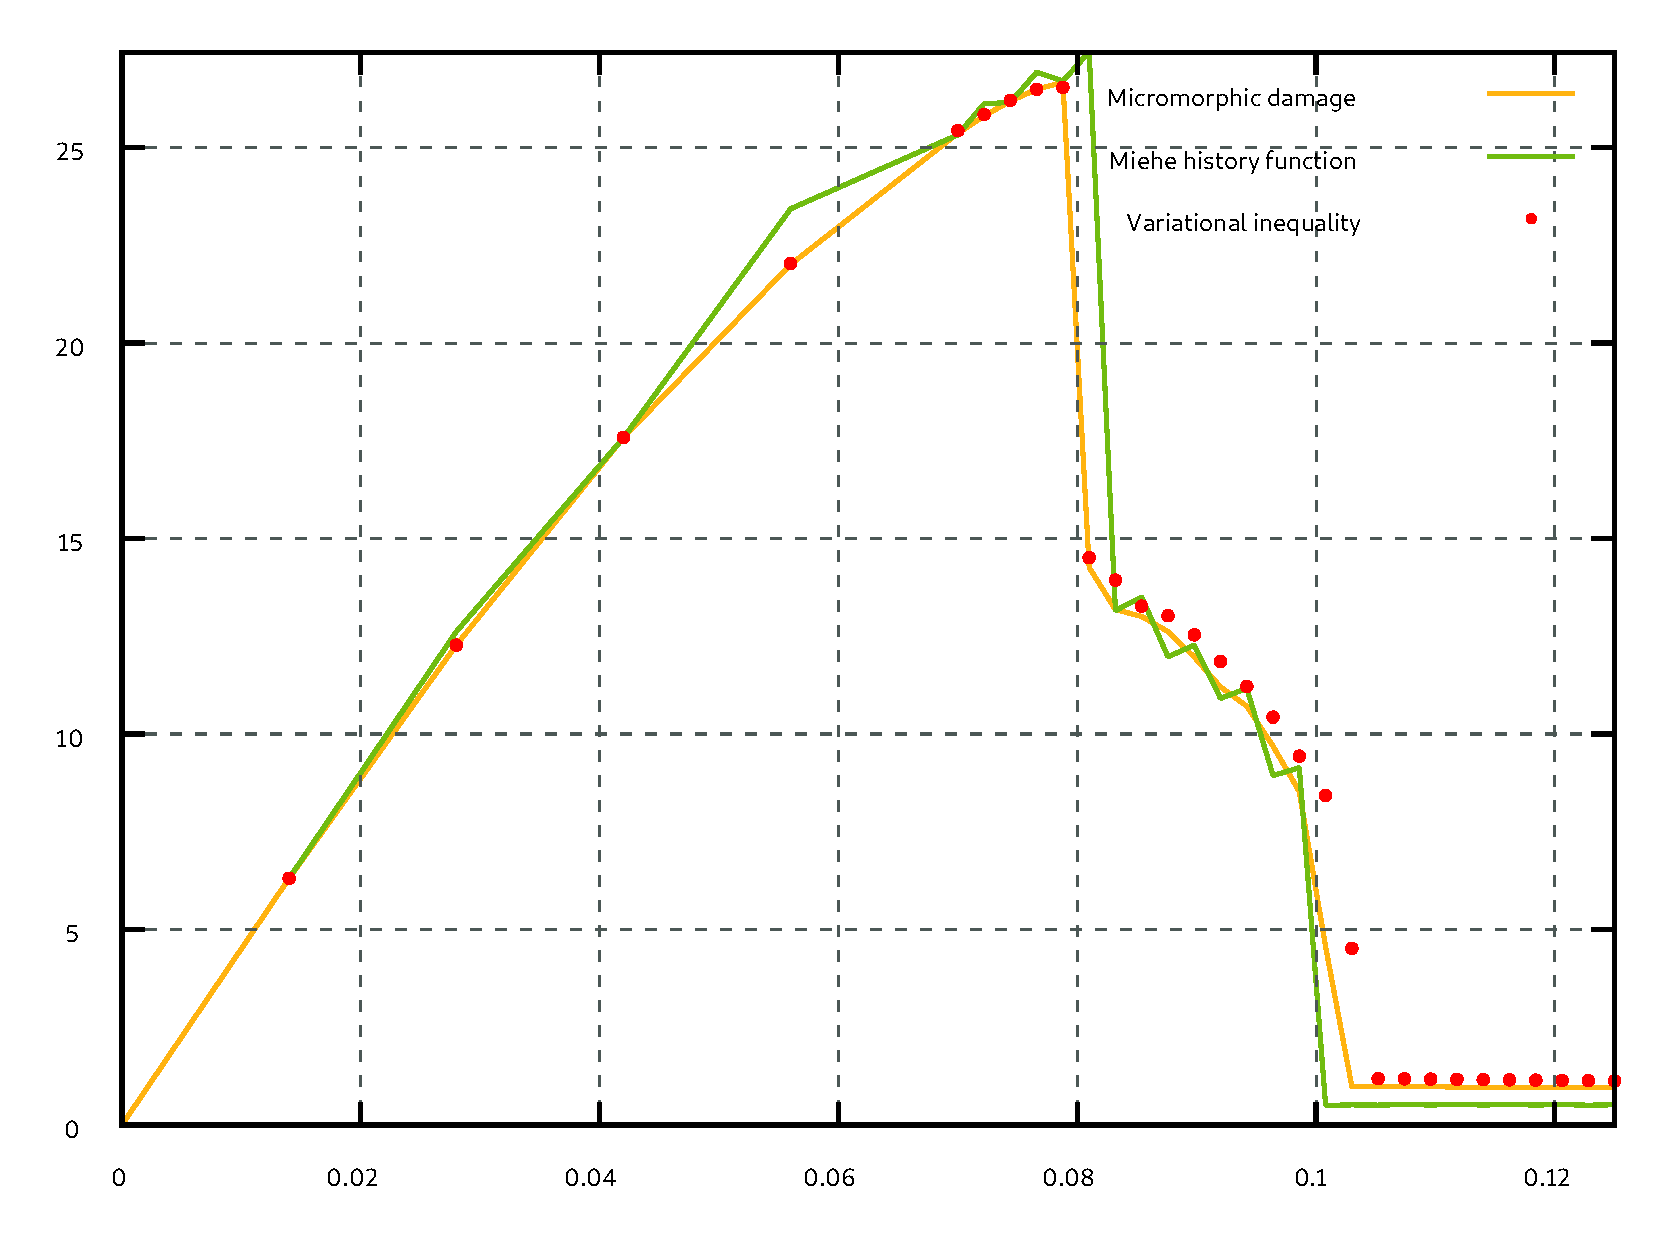
\includegraphics[width=10.cm]{../chapter_003_ef_micromorphic/figures/FiberReinforcedMatrix-force.pdf}
  \caption{Evolution of the force as a function of the imposed displacement for
  the fiber reinforced matrix test for the third scheme with \(\beta=150\)
  and the standard phase-field schemes based on the resolution of the
  variational inegality or based on Miehe' history
  function \cite{miehe_phase_2010}}
  \label{fig:micromorphic_damage:force}
\end{figure}

\subsection{Shear test on a notched plate}

\paragraph{Specimen and loading}

The second test case describes a square plate of length 1mm,
that is clamped at the bottom in the vertical direction (see Figure \ref{fig:micromorphic_formulation:shear_plate}).
A tangential displacement of amplitude 0.125mm is applied at the top of the specimen, and one of the vertices
of the plate is fixed to prevent rigid body motions in the tangential direction.

\begin{figure}[H]
    \centering
    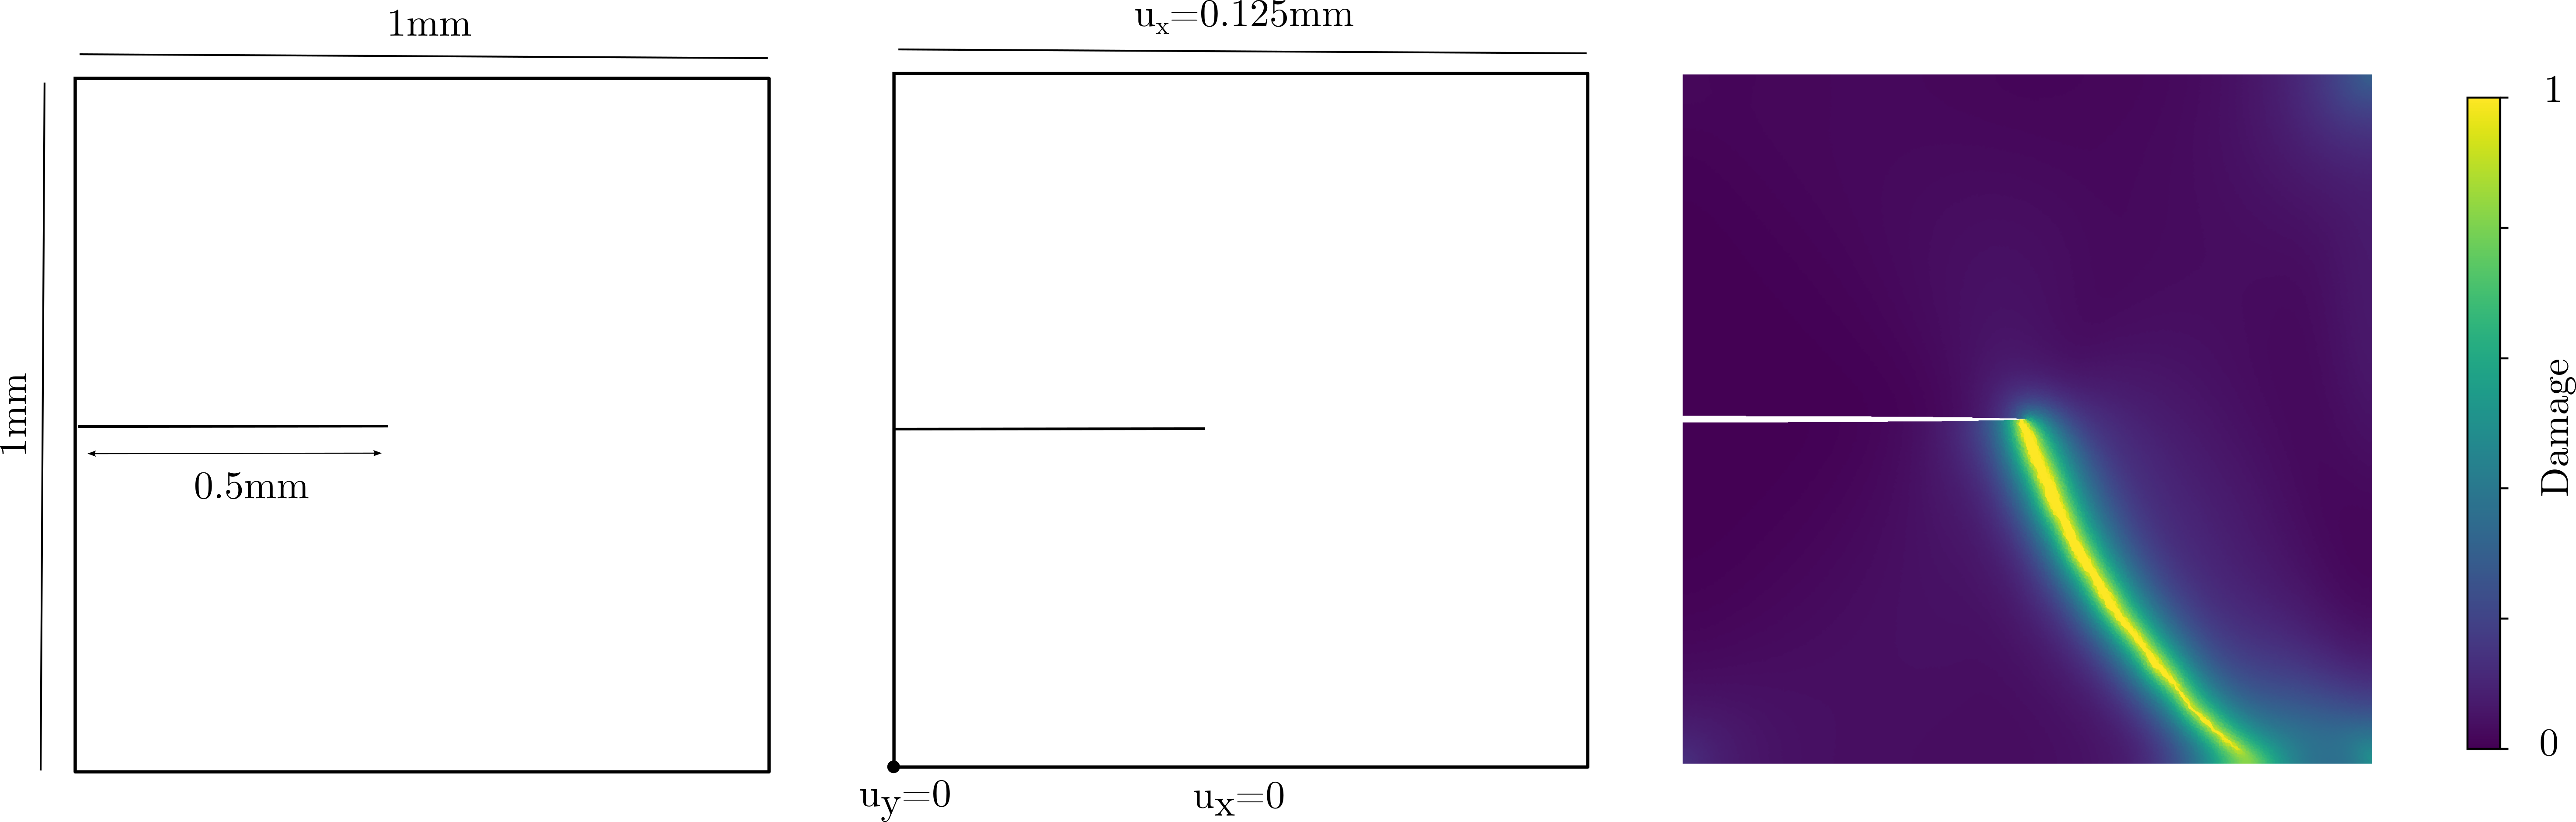
\includegraphics[width=14.cm]{../chapter_003_ef_micromorphic/drawings/shear_plate.png}
    \caption{Geometry, boundary conditions and damage pattern}
    \label{fig:micromorphic_formulation:shear_plate}
\end{figure}

\paragraph{Material behaviour}

As for the precedent test case, a linear elastic energy potential $\psi_{\tensoriis{\varepsilon}}$ is considered,
with a Young's modulus $E=200$ MPa and a Poisson's ratio $\nu=0.2$.
The chosen micromorphic damage is also described by Equations \eqref{eq:ef_micromorphic:formulation:AT2_link},
with a fracture energy release rate $G_c=1$ J/mm${}^2$, and a characteristic length $\ell_c = 0.02$ mm.
The degradation function acts on the spherical part of free energy potential (See Section \ref{sec:micromorphic:deviatori_split})

\paragraph{Force delfection curve}

Figure \ref{fig:micromorphic_damage:beta} displays the force-deflection curve of the shear test, for the
proposed micromorphic approach based on the third resolution scheme described in Section \ref{sec:micromorphic:third_scheme} for several values
of the penalization parameter $\beta$.
As illustrated by Figure \ref{fig:micromorphic_damage:beta}, the
penalization factor plays a major role on the overall
force-deflection curve. Experiments show that a value of
$\beta = 150$ leads to undistinguishable results with those obtains using the AT2 model based
on the resolution of the variational inequality to enforce damage irreversibility.

\begin{figure}[H]
  \centering
  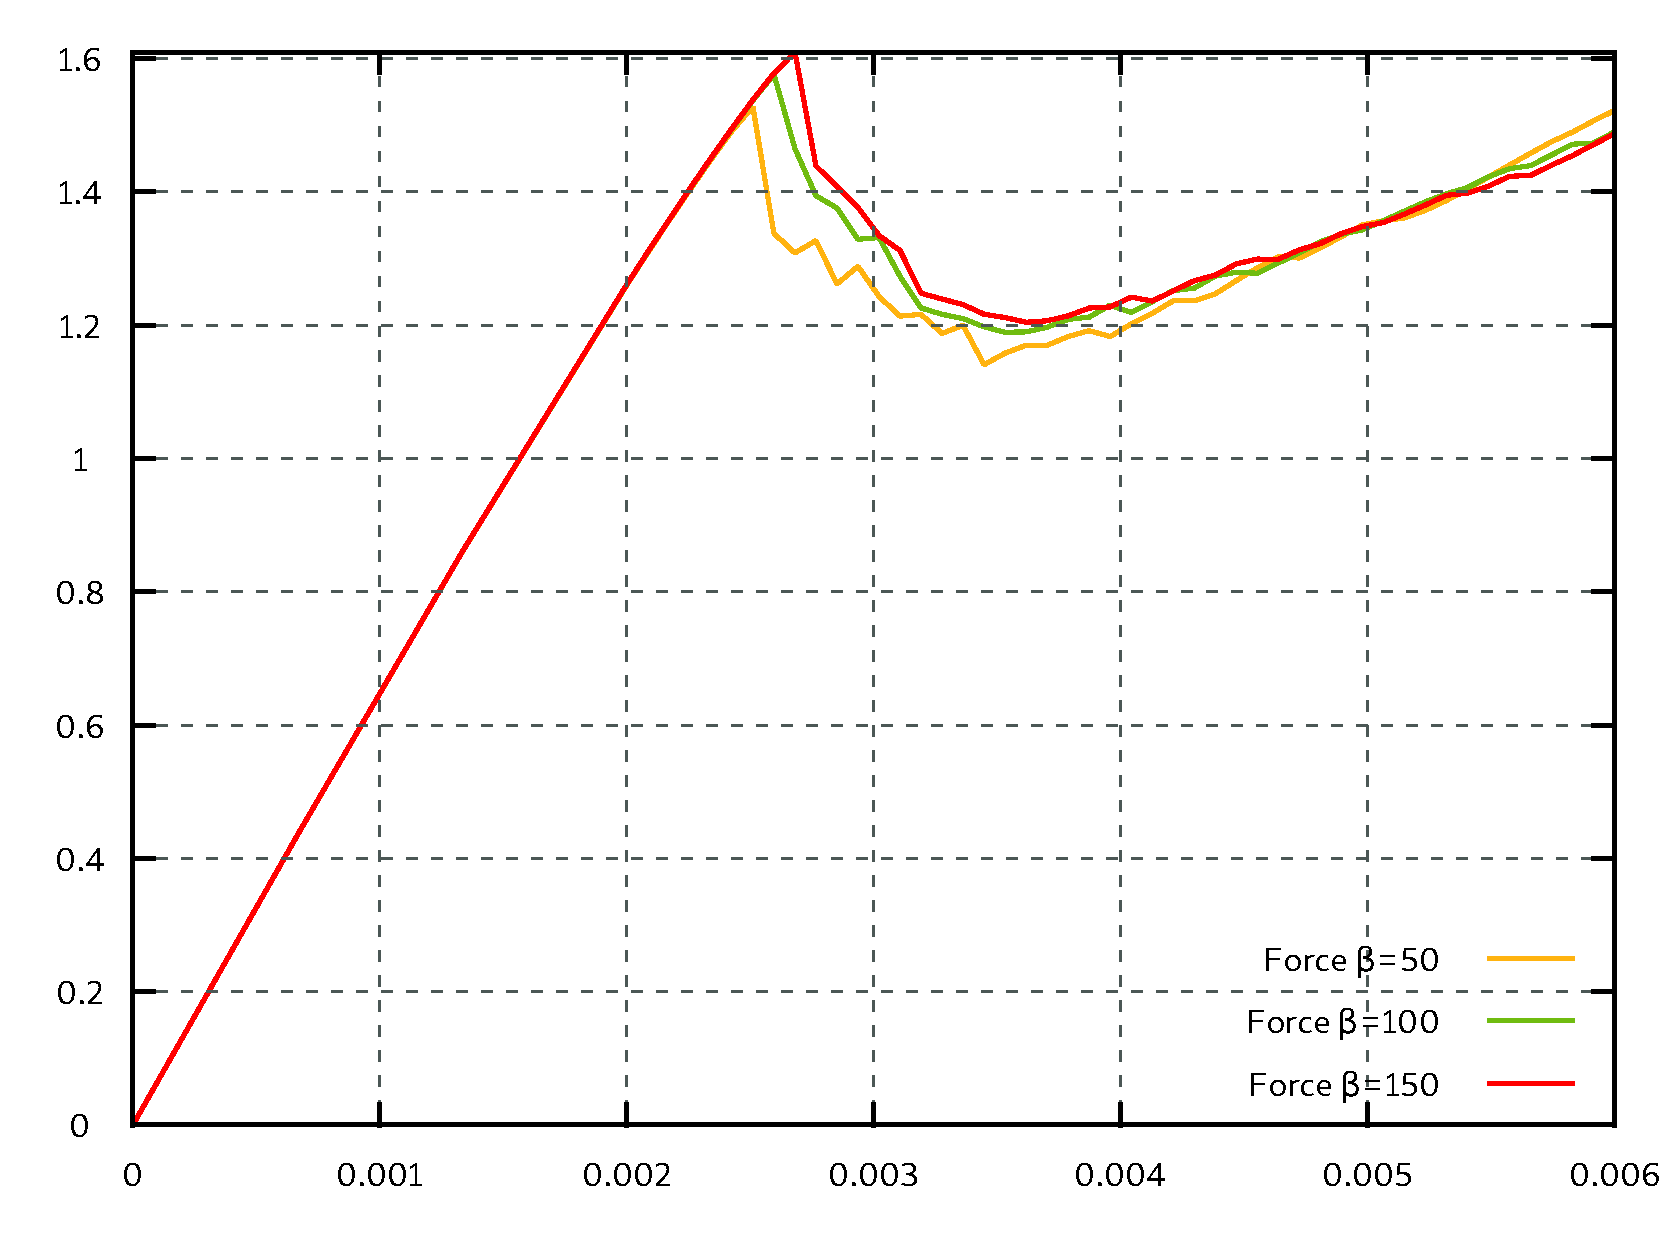
\includegraphics[width=10.cm]{../chapter_003_ef_micromorphic/figures/shear-force.pdf}
  \caption{Evolution of the force as a function of the imposed displacement for
  \(\beta=50\), \(\beta=100\), \(\beta=150\) for the shear test using the
  third staggered scheme}
  \label{fig:micromorphic_damage:beta}
\end{figure}

\paragraph{Number of iterations}

Figure \ref{fig:micromorphic_damage:shear:iterations} gives the number of iterations needed to achieve convergence of the fixed point algorithm
for the shear test, using the
proposed micromorphic approach based on the third resolution scheme, and for the AT2 phase field approach based on the resolution of the Karush–Kuhn–Tucker conditions
to enforce irreversibility of the damage field.
The number of iteration is roughly
similar between the standard AT2 model and the third scheme, although a
bit higher in general, as depicted on Figure
\ref{fig:micromorphic_damage:shear:iterations}.

\begin{figure}[H]
  \centering
  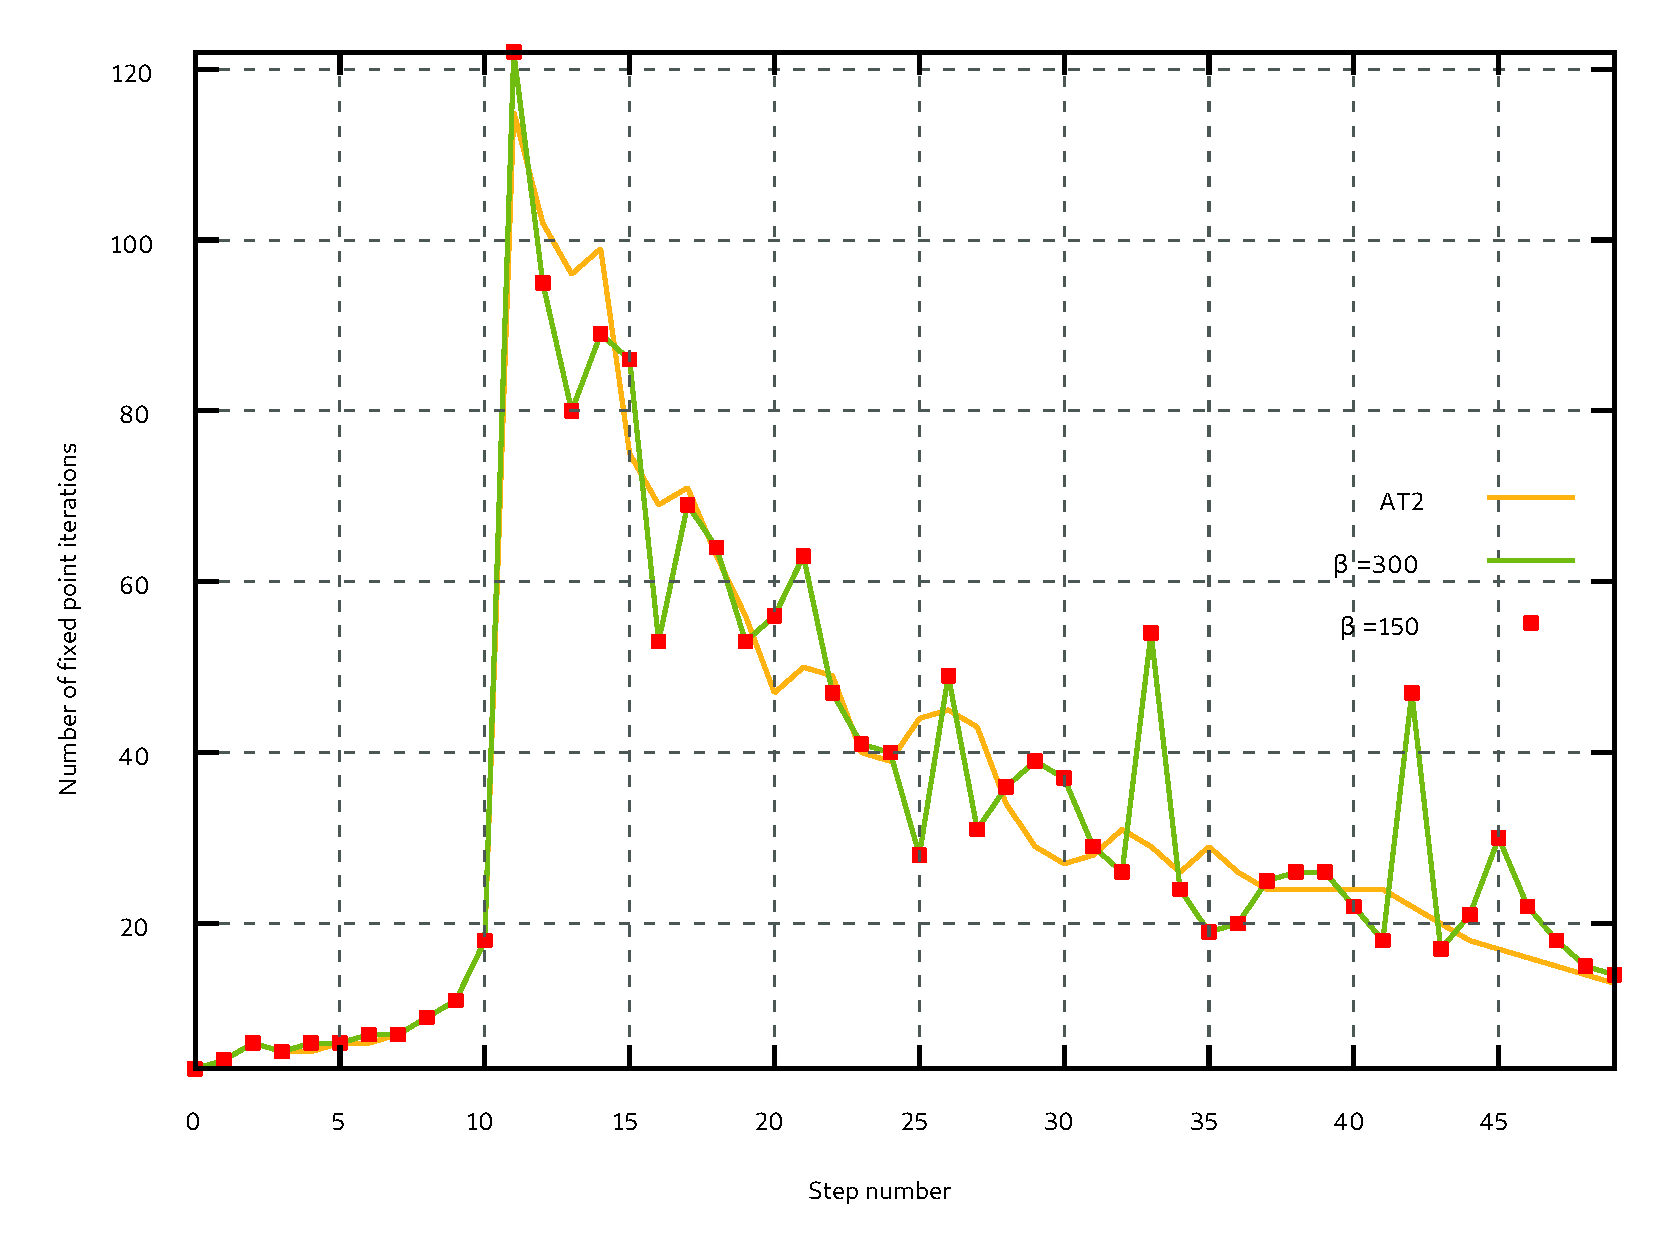
\includegraphics[width=10.cm]{../chapter_003_ef_micromorphic/figures/shear-iterations.pdf}
  \caption{Number of iterations of the fixed point algorithm for the shear test
  as a function of the step number for the standard AT2 model and the
  third scheme for \(\beta=150\) and
  \(\beta=300\)}
  \label{fig:micromorphic_damage:shear:iterations}
\end{figure}

% \paragraph{Coucou}

% However, an higher value of \(300\) is
% required to reproduce closely the evolution of the fracture energy.

\paragraph{Fracture energy}

Figure \ref{fig:micromorphic_damage:beta2} gives the evolution of the fracture energy as a function
of the imposed displacement, for the
proposed micromorphic approach and the third resolution scheme.
Values are compared to those obtained with the standard AT2 phase field model based the variational resolution of the evolution of damage.
A value of $\beta = 300$ is needed here to recover the energy dissipated by fracture for the AT2 model.

\begin{figure}[H]
  \centering
  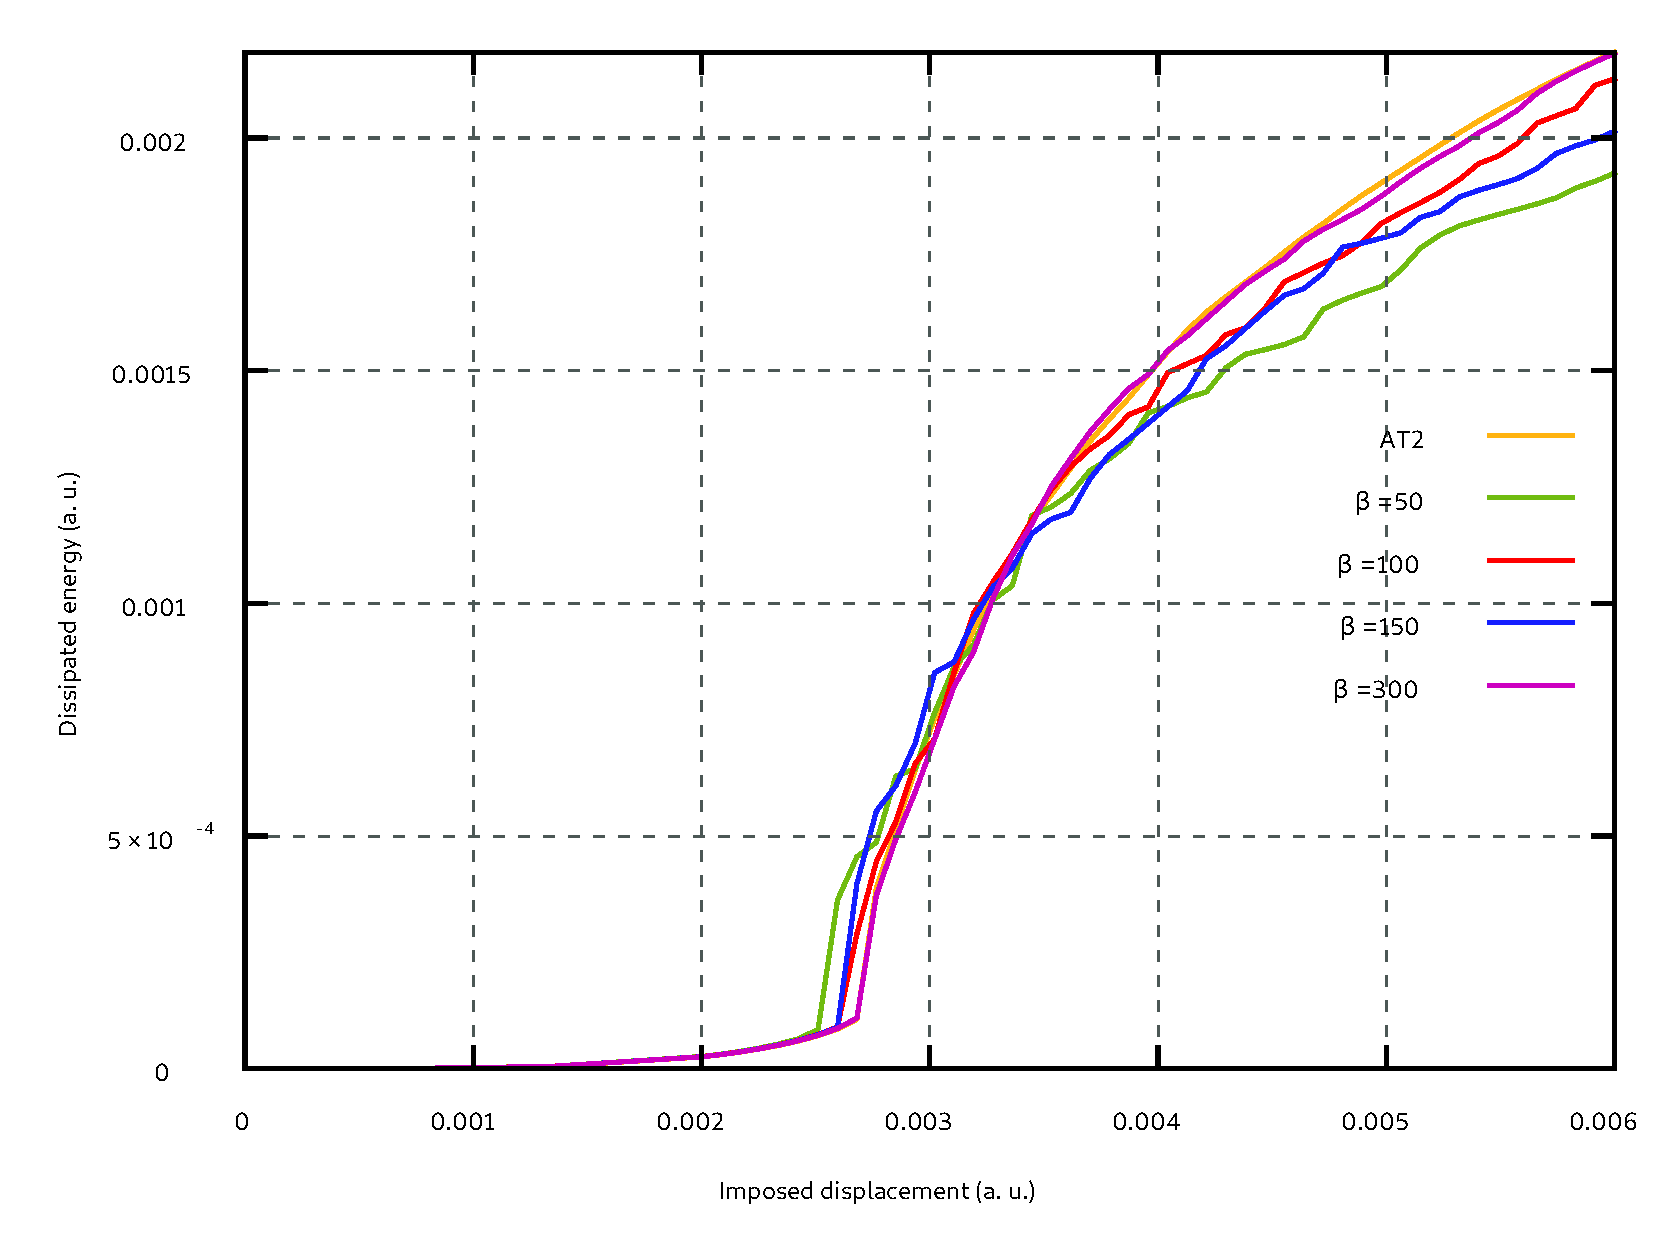
\includegraphics[width=10.cm]{../chapter_003_ef_micromorphic/figures/DissipatedEnergies.pdf}
  \caption{Evolution of the fracture energy as a function of the imposed
  displacement for \(\beta=50\), \(\beta=100\), \(\beta=150\) for the
  shear test using the third staggered
  scheme}
  \label{fig:micromorphic_damage:beta2}
\end{figure}

\subsection{Shear driven fracture on a tensile test}

\paragraph{Spaciemn and loading}

The considered test case taken from \cite{alessi_phase-field_2020} describes a simple rectangular rod
of length $2$mm and width $1$mm.
A vertical displacement of amplitude $0.125$mm is applied at the top of the specimen, and the
bottom is clamped in the vertical direction.
One of the vertices
of the plate is fixed in the tangential direction to prevent rigid body motions.
Natural
boundary conditions are considered elsewhere.

\begin{figure}[H]
  \centering
  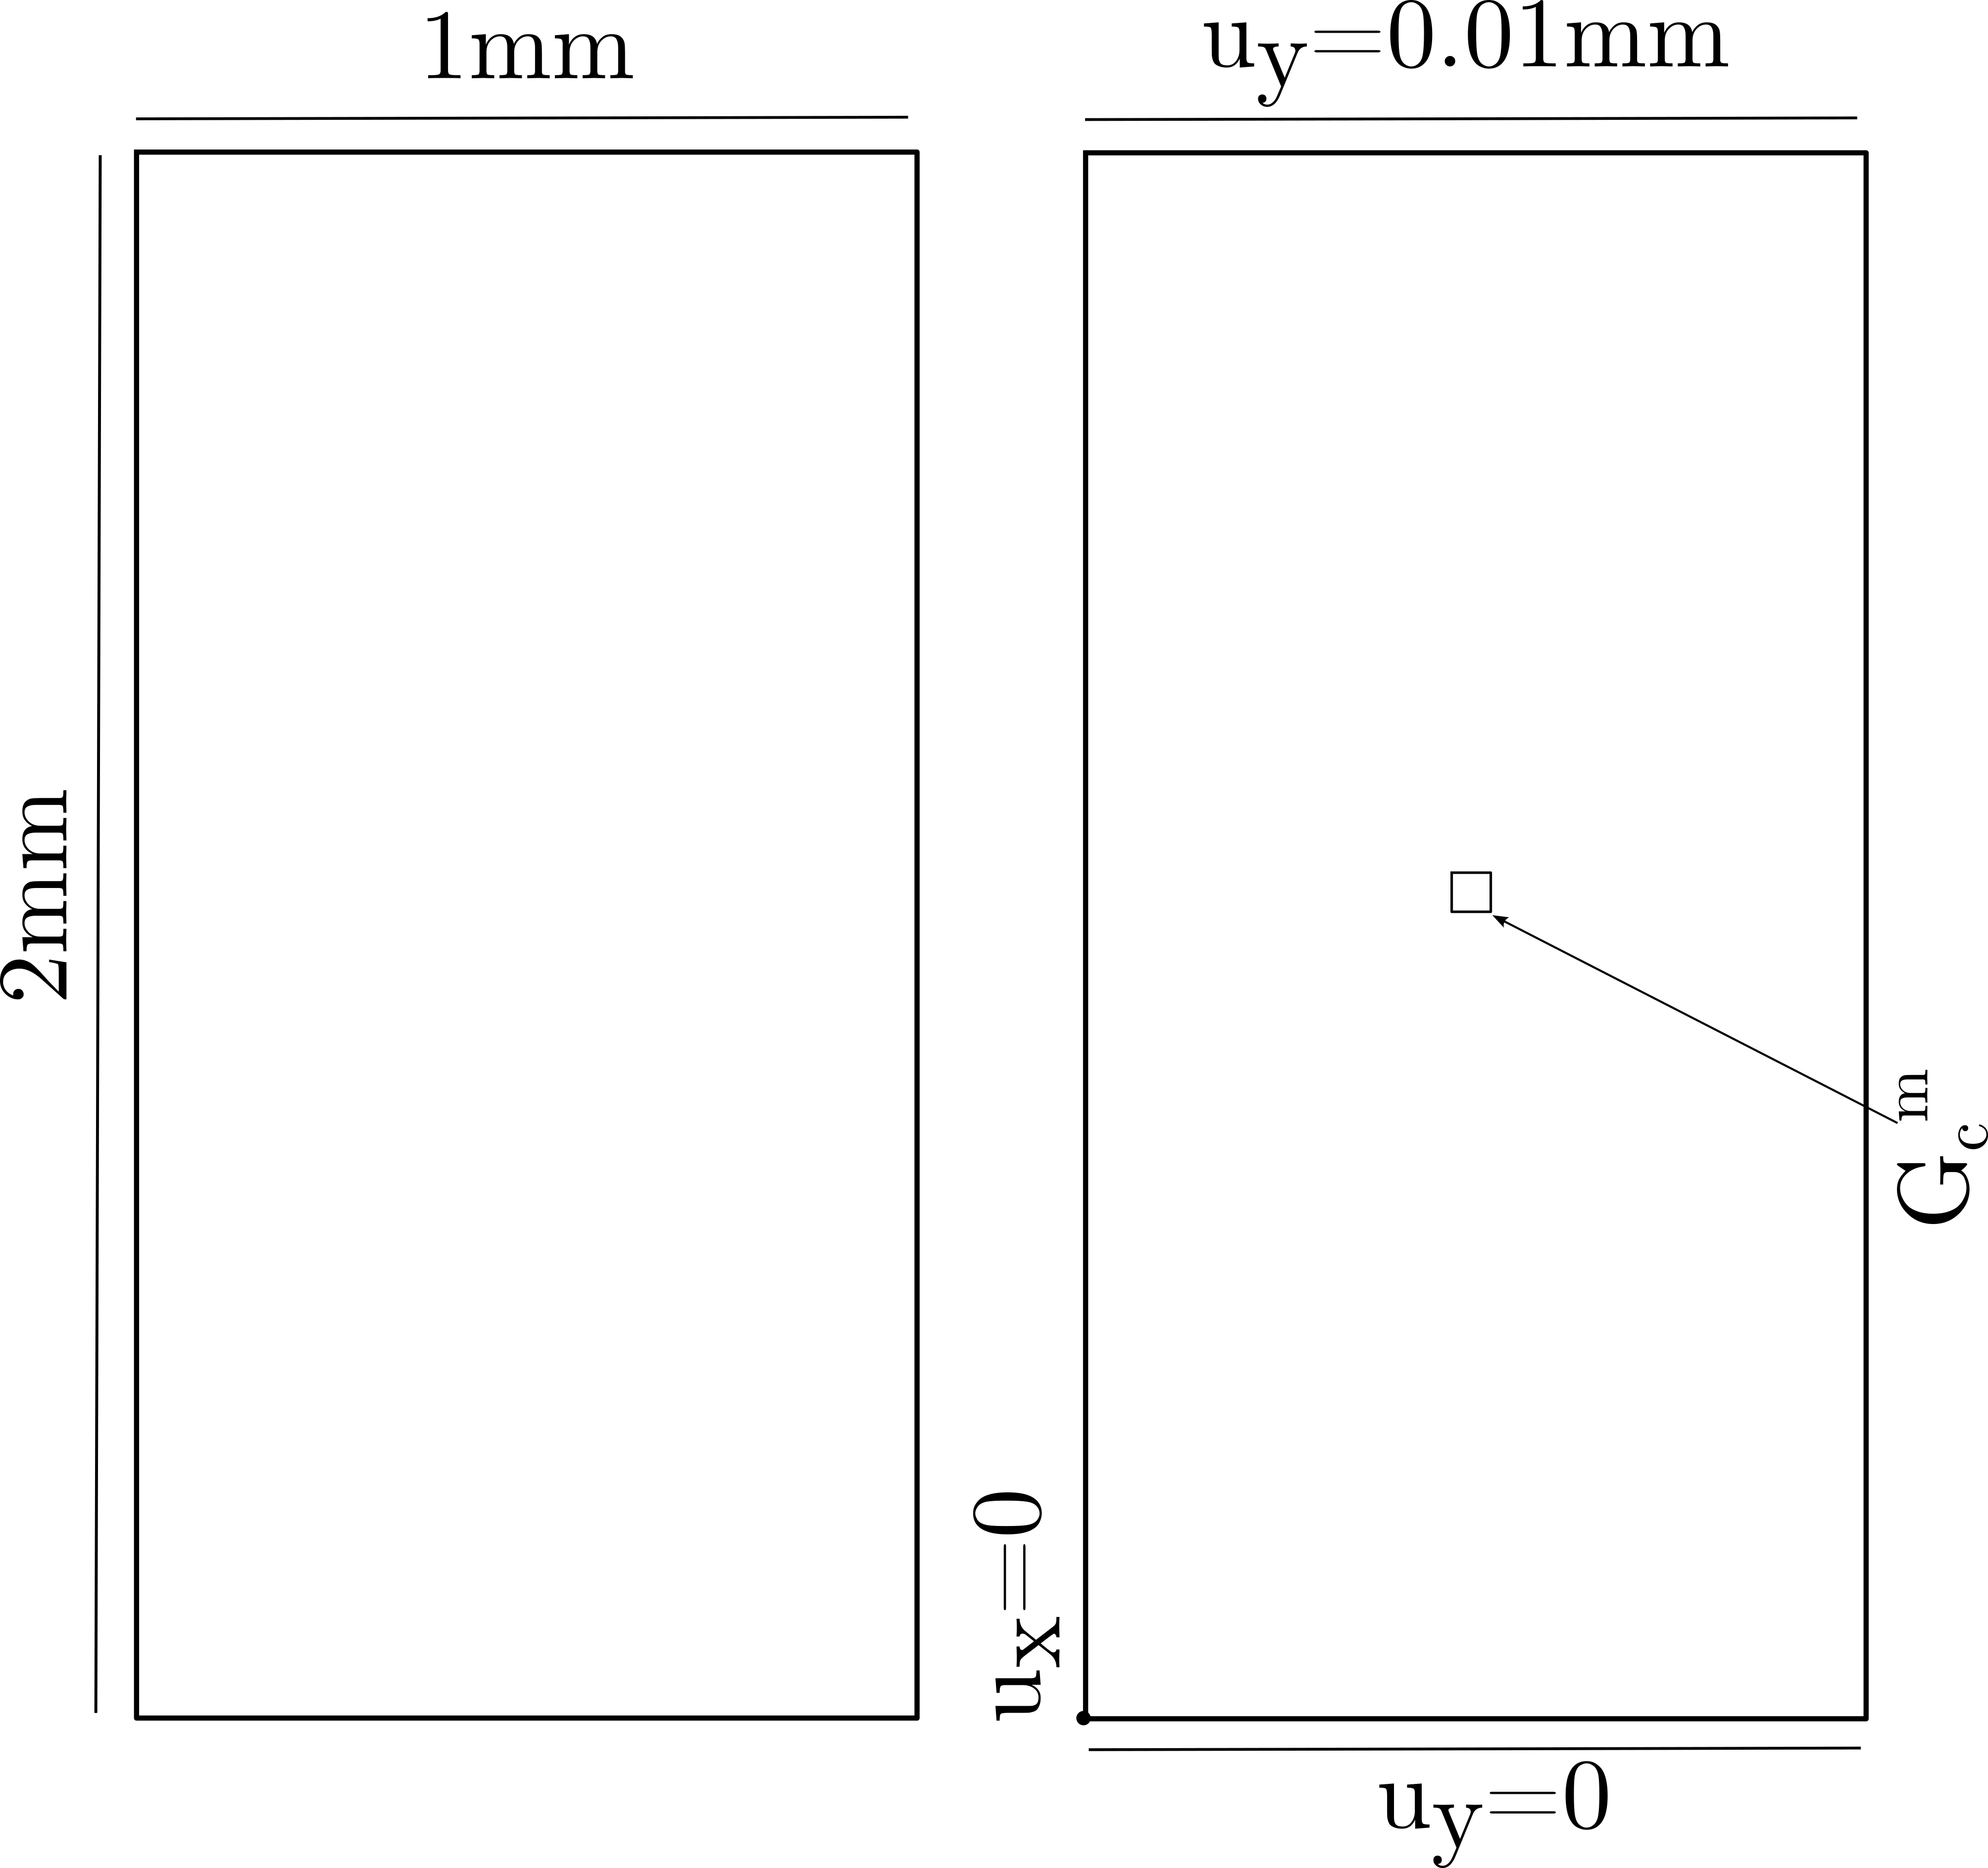
\includegraphics[width=8.cm]{../chapter_003_ef_micromorphic/drawings/alessi_mesh.png}
  \caption{Geometry, boundary conditions and defect zone for the shear driven fracture test case}
  \label{fig:micromorphic_damage:alessi_mesh}
\end{figure}

\paragraph{Material behaviour}

\textit{Alessi et al.} proposed a model to describe deviatoric driven fracture
using the following choice of the elastic free energy $\psi_{\tensoriis{\varepsilon}, \DamageField}$
%
%
%
\begin{equation}
  \psi_{\tensoriis{\varepsilon}, \DamageField}
  (\tensorii{\varepsilon}, \DamageField)
  =
  \frac{\mu}{2} \, g(\DamageField) \, \tensorii{\varepsilon}{}^{\text{dev}} : \tensorii{\varepsilon}{}^{\text{dev}}
  +
  \frac{K}{2} \, \tensorii{\varepsilon}{}^{\text{sph}} : \tensorii{\varepsilon}{}^{\text{sph}}
\end{equation}
%
%
%
where $K = 175$ GPa is the bulk modulus, $\mu = 80.77$ Gpa is the shear modulus, $\tensorii{\varepsilon}{}^{\text{dev}}$ is the
deviatoric part of the elastic strain, and $\tensorii{\varepsilon}{}^{\text{sph}}$ is the spherical
part.
The chosen micromorphic damage is described by Equations \eqref{eq:ef_micromorphic:formulation:AT2_link},
with a fracture energy release rate $G_c=2.7$ J/mm${}^2$, and a characteristic length $\ell_c = 0.025$ mm.
For damage initiation to localize at the center of the specimen, a degraded fracture energy release rate $G_c^{m}=0.99 G_c$
is imposed in a square of size $0.05$mm at the middle of the rod.

\paragraph{Quasi-incompressible behaviour}

As stated by \textit{Alessi et al.}, this model leads to quasi-incompressible
behaviour in highly damaged zones, and Lagrange elements are not able to
properly describe the damage localization band as well as the energy dissipated
by the crack propagation. They then showed that various
classical approaches (selective reduced integration and mixed
displacement/pressure formulation) can overcome this issue.
%
%
%
This test case is adapted to demonstrate that the
micromorphic approach can be used with higher order finite elements in order to alleviate this issue.
In the following, the same order of approximation are used to solve both the mechanical and
the micromorphic problems.

\paragraph{Mesh description}
The rod is discretized with triangle elements. The number of elements
used as a function of the finite element order is given in Table
\ref{tbl:micromorphicdamage:shear_driven_fracture_test_elements}. In
practice, the number of elements have little influence on the results
and the conclusions drawn in the next paragraph.
A very fine
mesh is used for low order finite elements (\(1\) and \(2\)) with
several dozen elements inside the damage band (See Figure
\ref{fig:micromorphicdamage:shear_driven_fracture_test_order1}). A coarser
mesh is used for higher order elements (\(4\) and \(6\)) with \(4\) to
\(6\) elements inside the damage band.
%
%
%
\begin{table}[H]
  \centering
  \begin{tabular}{||c c||} 
      \hline
      Resolution Method & Memory footprint
      \\
      [0.5ex] 
      \hline\hline
      Order 1 & \(102\,272\) elements
      \\ \hline
      Order 2 & \(409\,088\) elements
      \\ \hline
      Order 4 & \(25\,568\) elements 
      \\ \hline
      Order 6 & \(25\,568\) elements 
      \\ \hline
  \end{tabular}
  \caption{Geometry and material parameters for the shear driven fracture test}
  \label{tbl:micromorphicdamage:shear_driven_fracture_test_elements}
\end{table}

\paragraph{Damage pattern for low order elements}

Figure \ref{fig:micromorphicdamage:shear_driven_fracture_test_order1}
describes the damage pattern after the propagation of the crack. As
described by \textit{Alessi et al.}, volumetric locking leads to a spurious
damage localization band with excessive thickness, \textit{i.e.} a thickness
largely greater than the characteristic length \(\ell_{c}\). A very fine
mesh is used to demonstrate that the issue is not solved by mesh
refinement.

\begin{figure}[H]
  \centering
  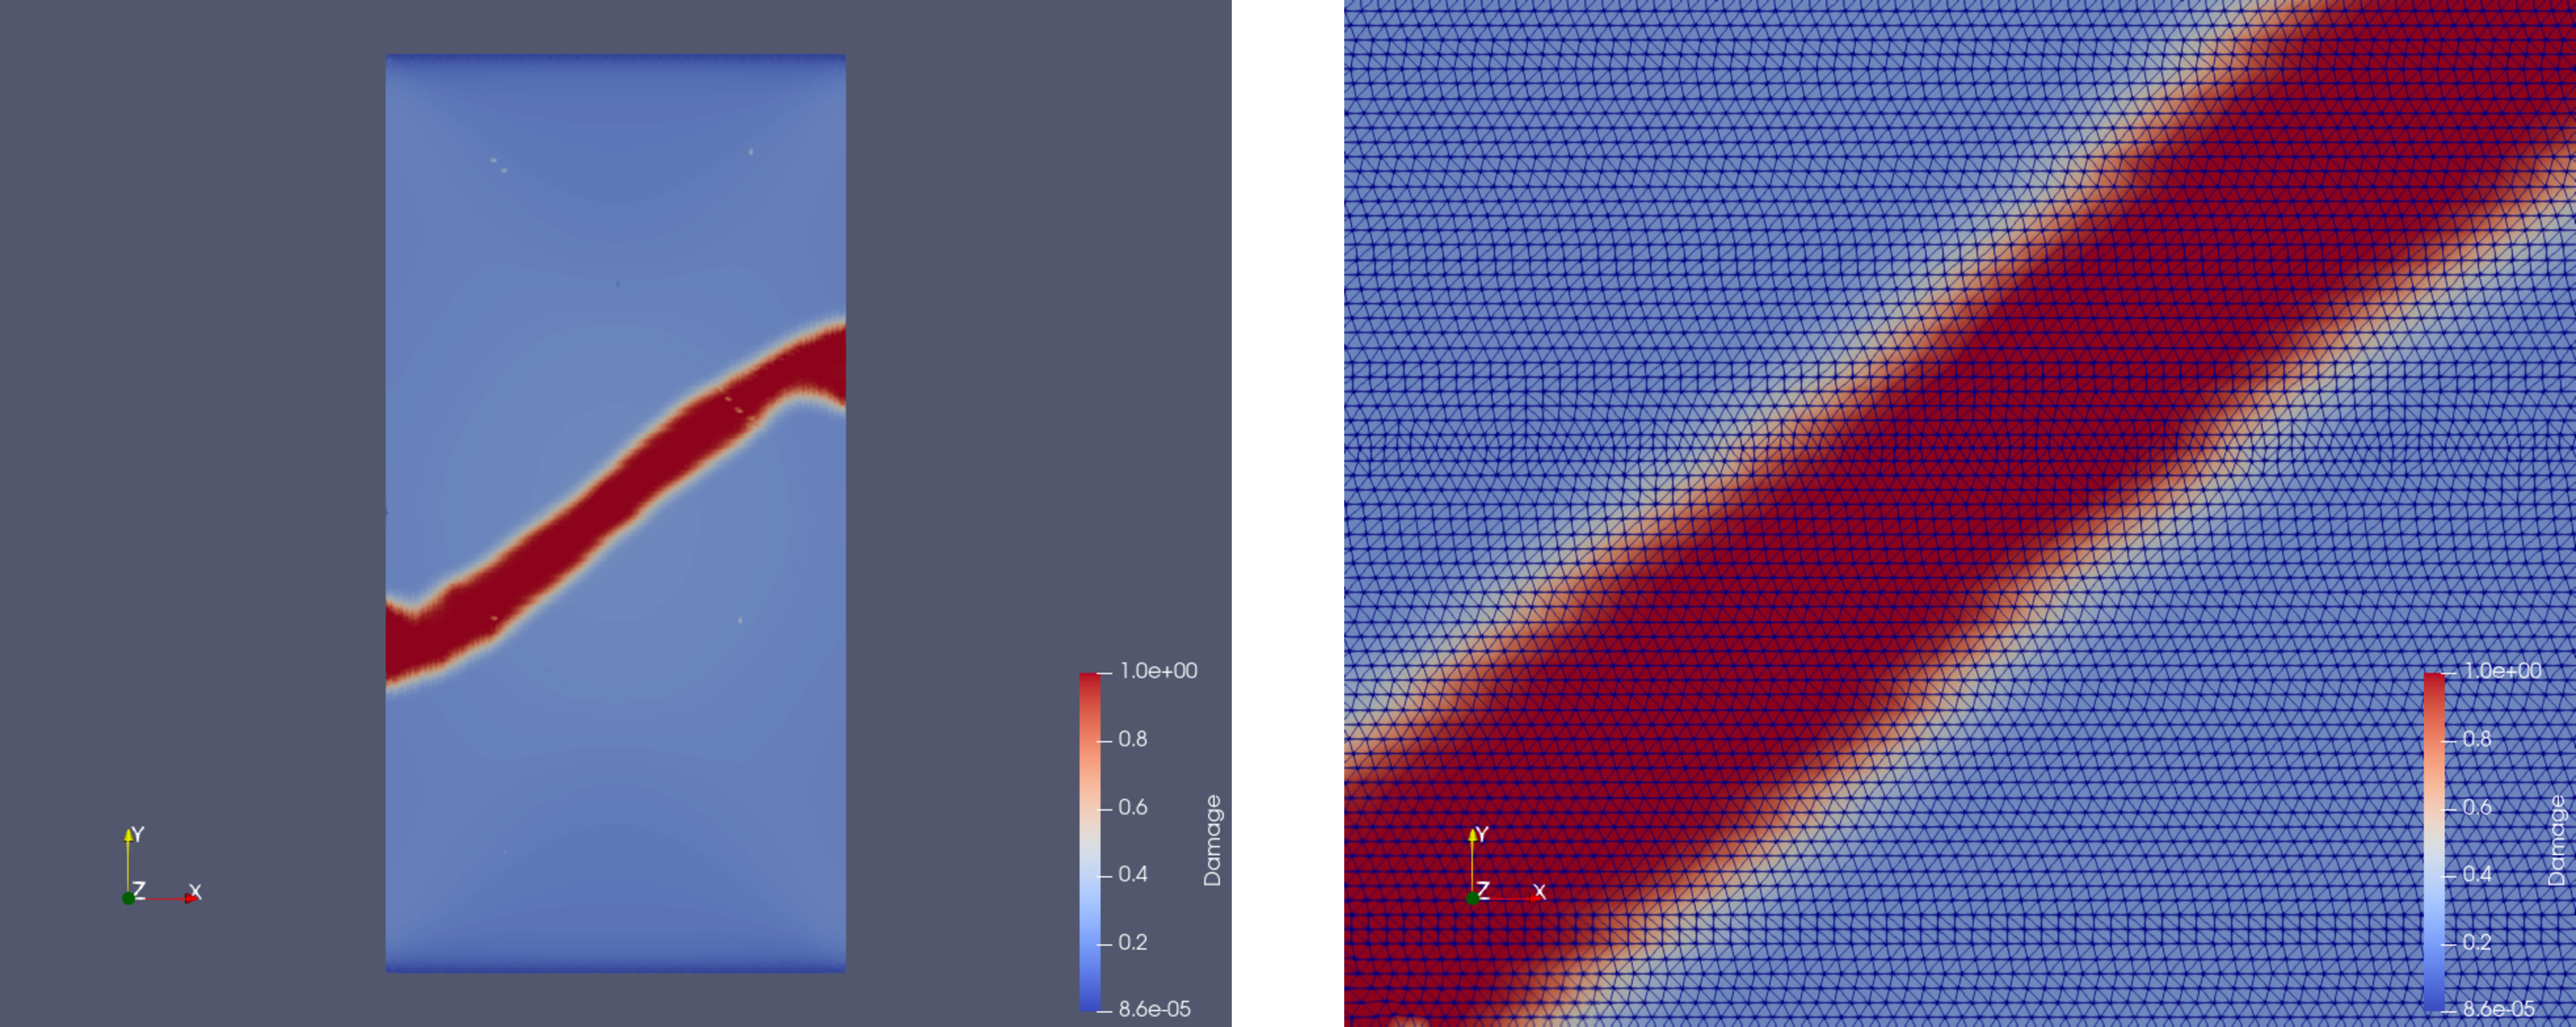
\includegraphics[width=14.cm]{../chapter_003_ef_micromorphic/figures/shear-driven-fracture-damage-results-order-1.pdf}
  \caption{Spurious damage map obtained with linear elements (left). Zoom on the shear fracture (right)}
  \label{fig:micromorphicdamage:shear_driven_fracture_test_order1}
\end{figure}

\paragraph{Damage pattern for high order elements}

Figure \ref{fig:micromorphicdamage:shear_driven_fracture_test_higher_order}
show the results obtained with higher order elements. While the
simulation with quadratic elements still exhibit a spurious damage
localisation band, similar to the one observed with linear elements in
Figure \ref{fig:micromorphicdamage:shear_driven_fracture_test_order1}, higher
order elements lead to satisfying results, i.e. higher order elements
alleviate issues related to volumetric locking.

\begin{figure}[H]
  \centering
  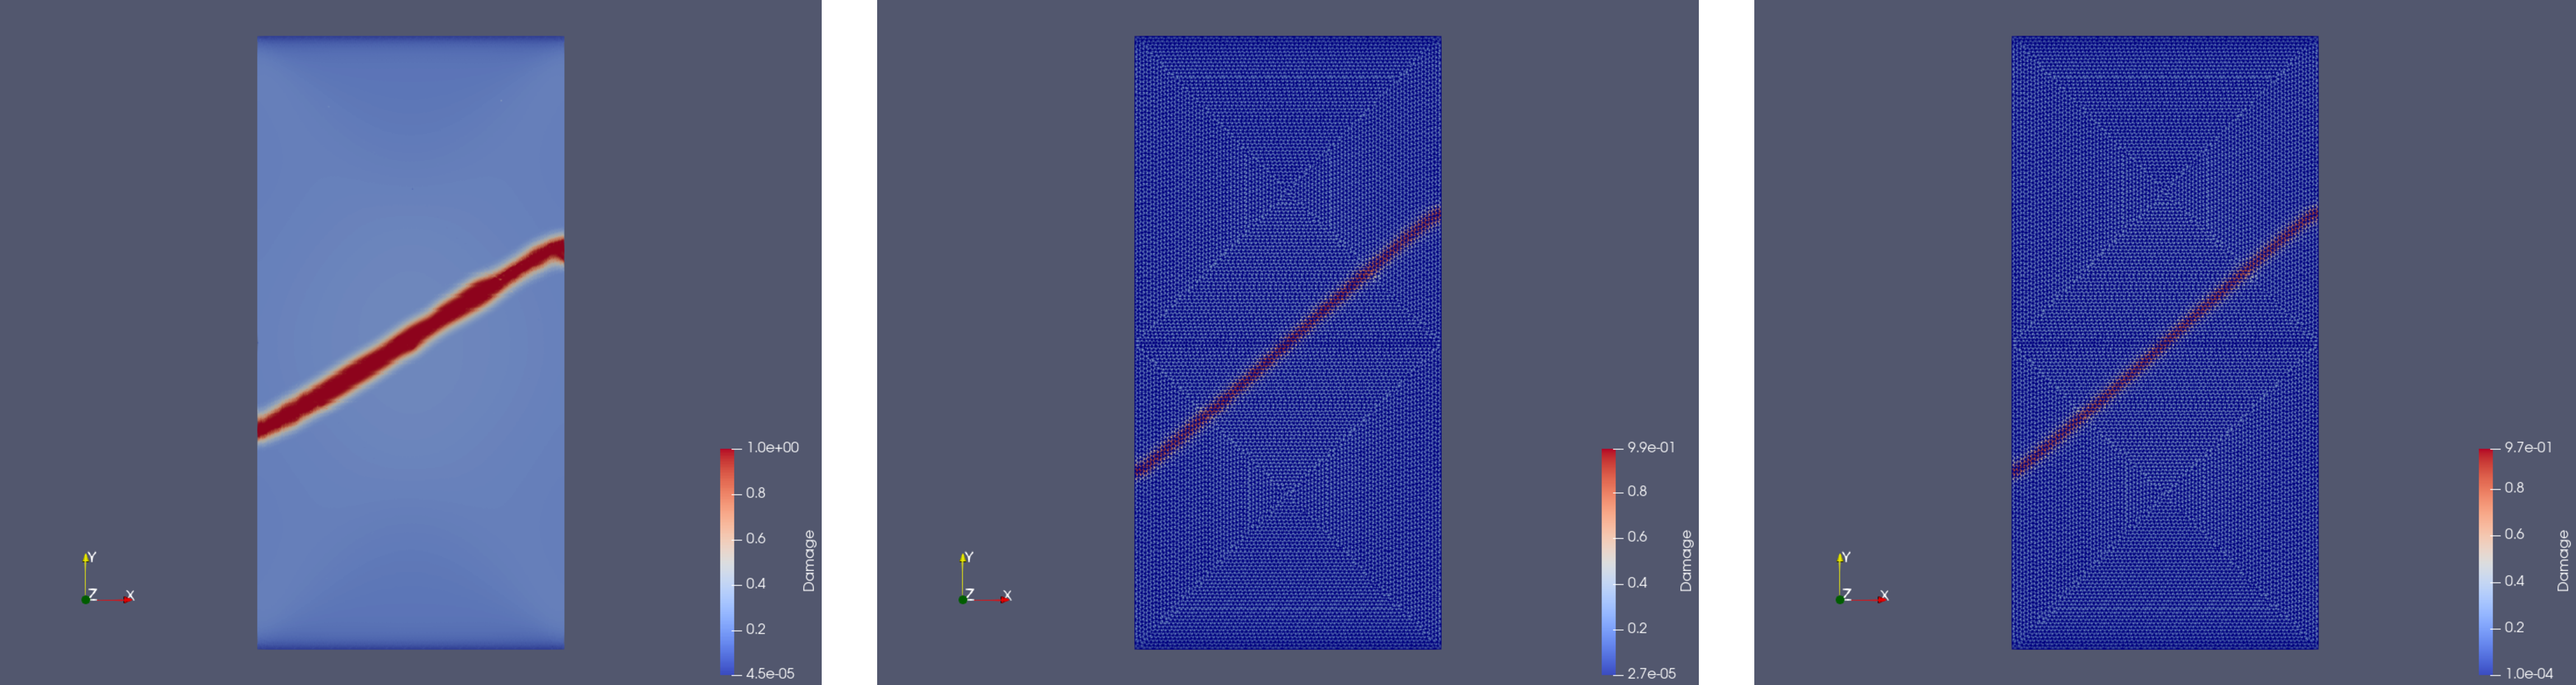
\includegraphics[width=14.cm]{../chapter_003_ef_micromorphic/figures/shear-driven-fracture-damage-results-higher-orders.pdf}
  \caption{Damage map for higher order elements. Quadradic elements (left), fourth order elements (center), sixth order elements (right). The quadratic mesh is too fine to be shown without hiding the results}
  \label{fig:micromorphicdamage:shear_driven_fracture_test_higher_order}
\end{figure}

\paragraph{Force deflection curves}

Figure \ref{fig:micromorphicdamage:traction_curve} presents the
force/displacement curves as a function of the finite element order.
Quadratic results, which are intermediate between linear and quadratic
results, are not reproduced for the sake of clarity.

\begin{figure}[H]
  \centering
  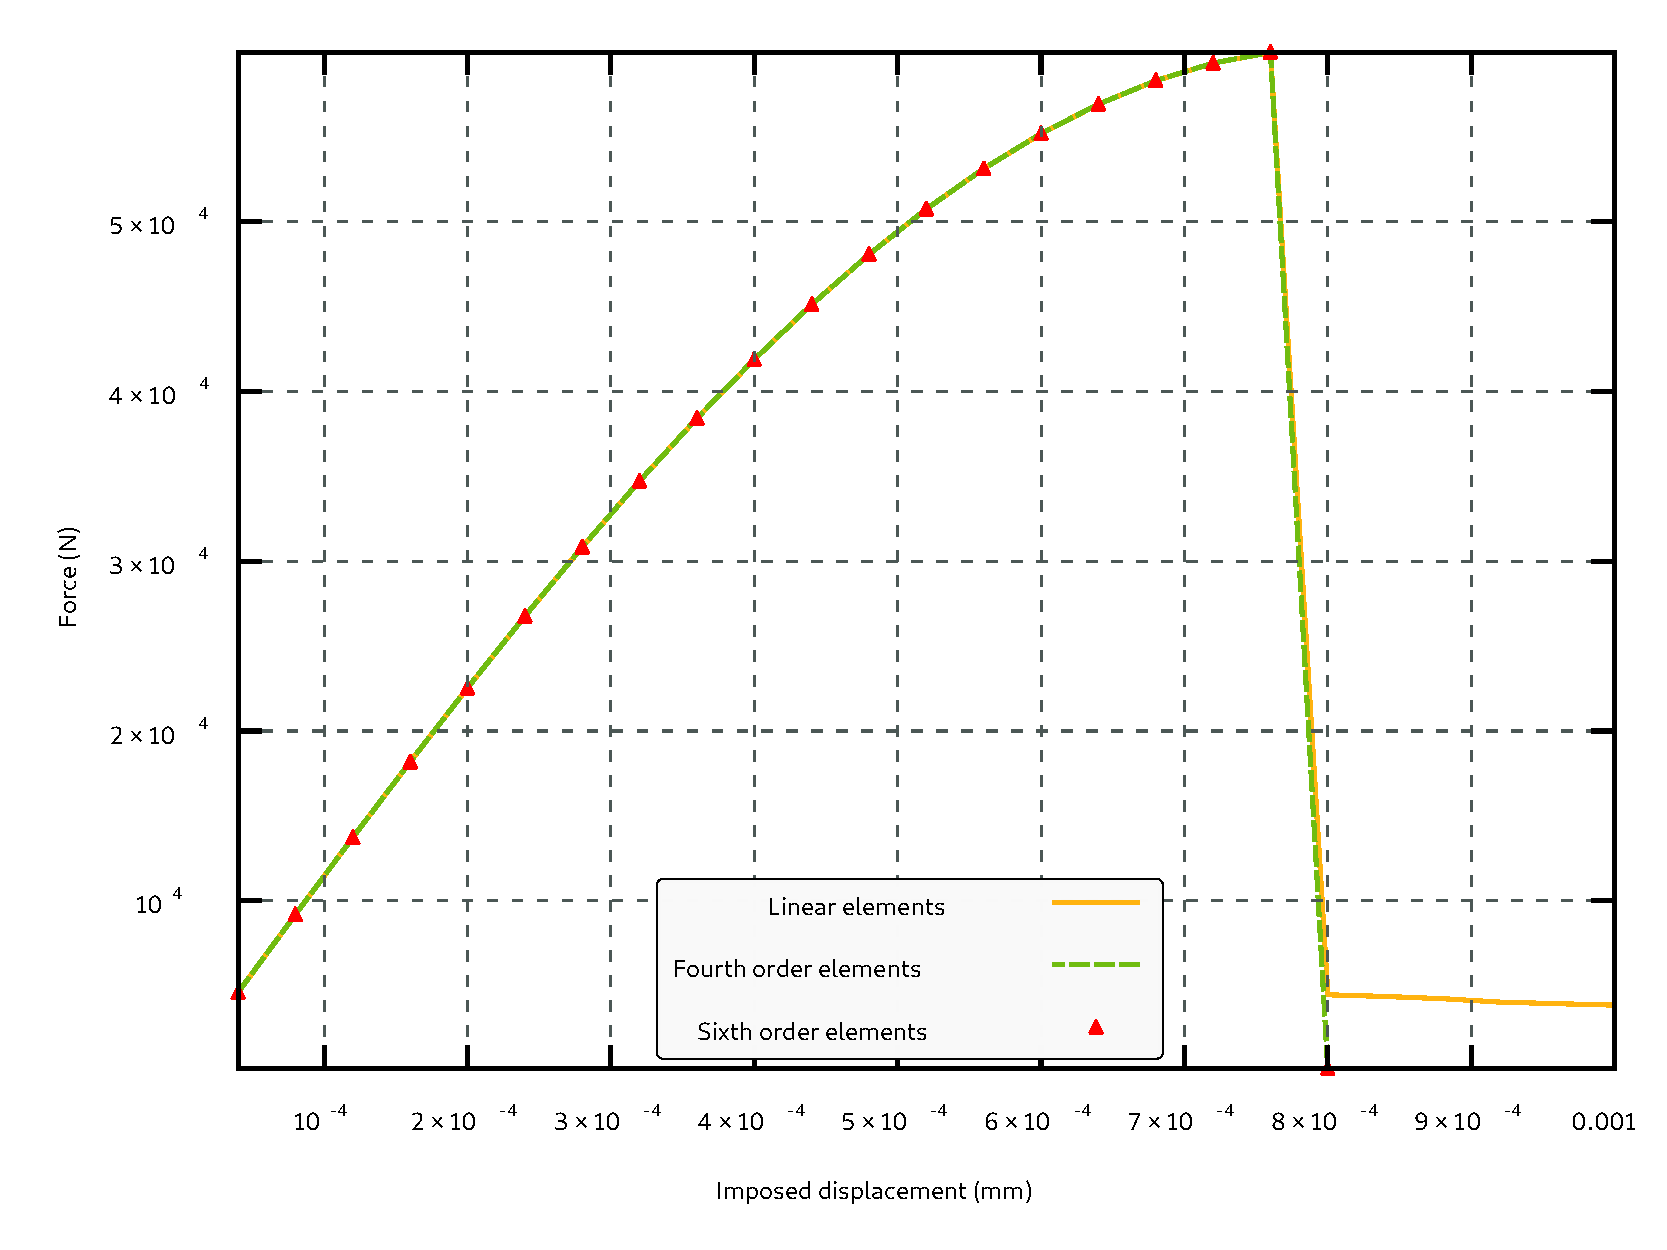
\includegraphics[width=10.cm]{../chapter_003_ef_micromorphic/figures/shear-driven-fracture-damage-results-force.pdf}
  \caption{Traction curve}
  \label{fig:micromorphicdamage:traction_curve}
\end{figure}

\paragraph{Observations}

All order of approximations give similar results up to the crack propagation.
The traction curve given by linear elements exhibits a residual
stiffness and a spurious dissipation after the crack propagation.
Fourth order and sixth order give undistinguishable results. In both
cases, the force drops to zero after the crack propagation.

\subsection{Fragmentation of a nuclear fuel pellet}

\paragraph{Spaciemn and loading}

This test case describes the fragmentation of a nuclear fuel pellet during the
reactor start-up.
The pellet is a cylinder of width $8.17$mm and height $13.4$mm.
The top and bottom surfaces are recessed by a dishing of diameter $6.1$mm and height $0.32$mm.
The pellet is fixed at one point to prevent rigid body motions.
Assuming a constant thermal conductivity, a temperature load $T(r, t)$ is imposed in the pellet such that
%
%
%
\begin{equation}
  T(r, t) = (T_{\mathrm{c}} - T_{\mathrm{o}}) t \, (1-r^{2}) + T_{\mathrm{o}}
\end{equation}
%
%
%
where $T_{c} = 1500$K is the core temperature, $T_{o} = 600$K is the outer surface temperature,
and $r$ is the radial component such that $r=0$ on the symmetry axis of the pellet, and $t$ is a
pseudo-time loading parameter in the range \([0,1]\).
%
%
%

% The considered test case taken from \cite{alessi_phase-field_2020} describes a simple rectangular rod
% of length $2$mm and width $1$mm.
% A vertical displacement of amplitude $0.125$mm is applied at the top of the specimen, and the
% bottom is clamped in the vertical direction.
% One of the vertices
% of the plate is fixed in the tangential direction to prevent rigid body motions.
% Natural
% boundary conditions are considered elsewhere.

\begin{figure}[H]
  \centering
  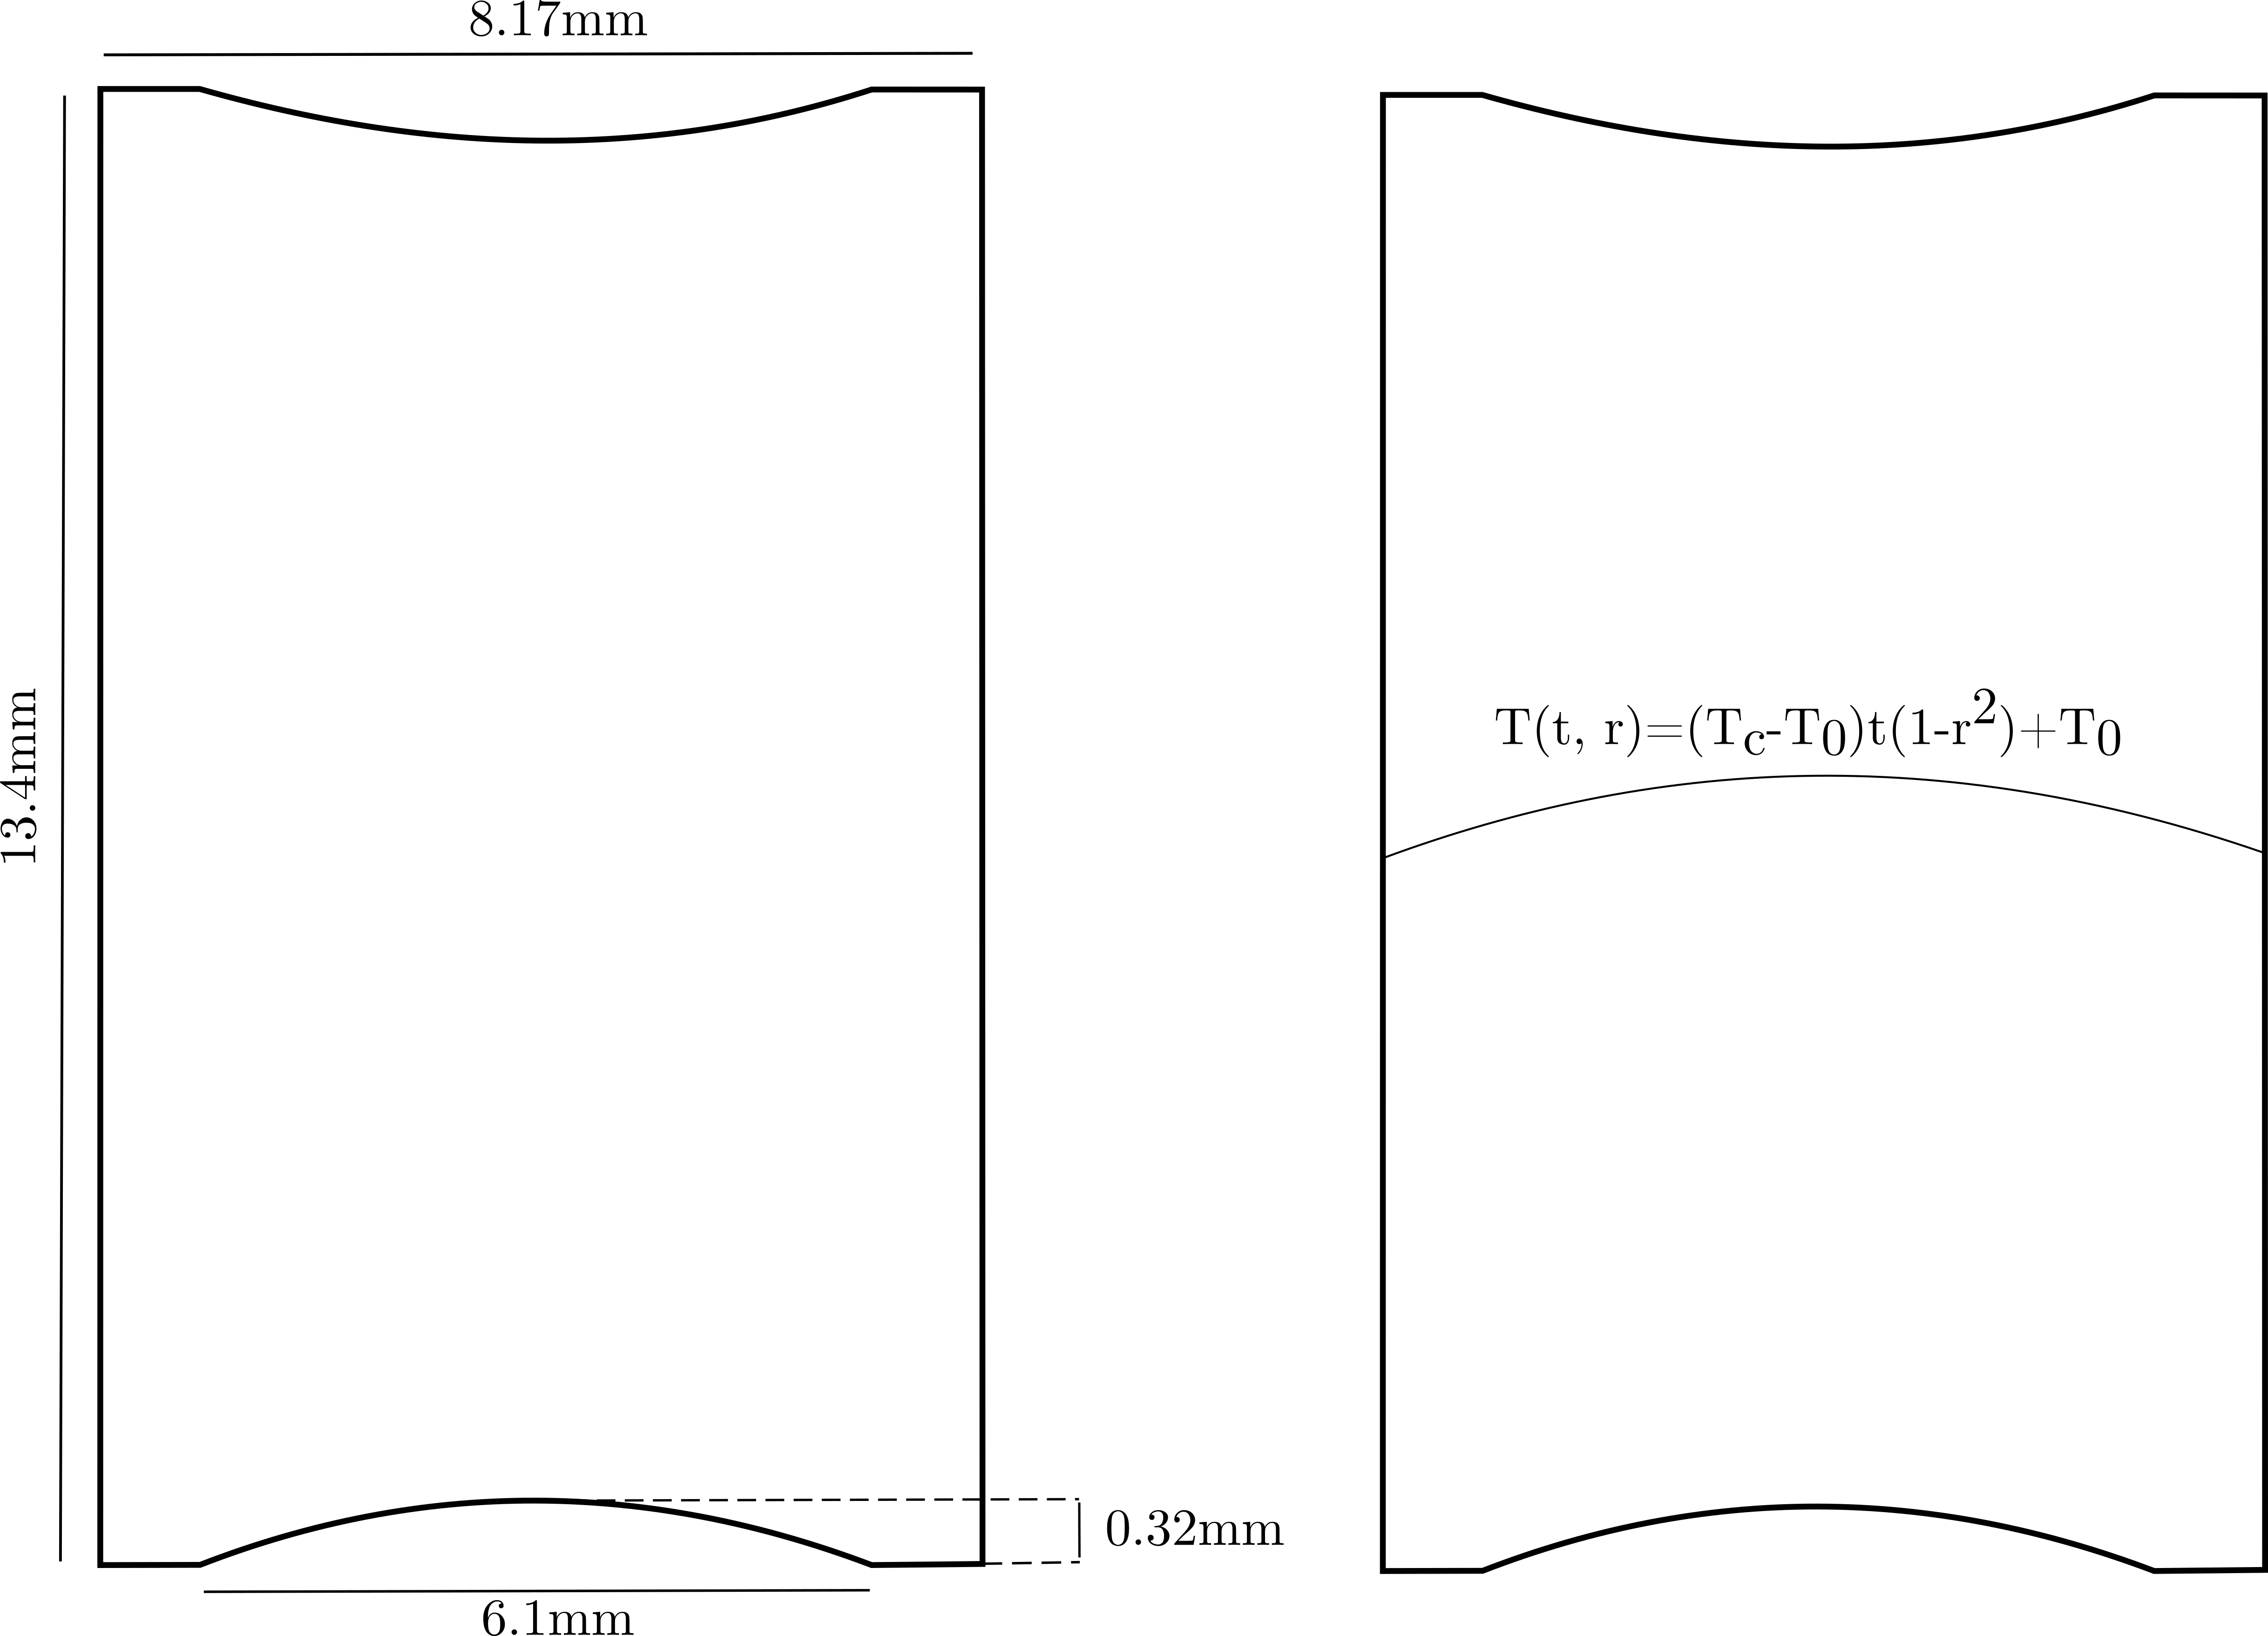
\includegraphics[width=10.cm]{../chapter_003_ef_micromorphic/drawings/pellet_mesh.png}
  \caption{Geometry, boundary conditions and defect zone for the pellet}
  \label{fig:micromorphic_damage:pellet_mesh}
\end{figure}

\paragraph{Material behaviour}

A linear thermo-elastic free energy potential is considered, such that
%
%
%
\begin{equation}
  \label{eq:micromorphicdamage:freeenergygel_2}
  \psi_{\tensoriis{\varepsilon}, \DamageField}
  (\tensorii{\varepsilon}, \DamageField, T)
  =
  g(\DamageField) \, \psi_{\tensoriis{\varepsilon}}^{\text{th}}(\tensorii{\varepsilon}, T)
\end{equation}
%
%
%
where the thermo-elastic potential $\psi_{\tensoriis{\varepsilon}}^{\text{th}}$ is such that
%
%
%
\begin{equation}
  \psi_{\tensoriis{\varepsilon}}^{\text{th}}(\tensorii{\varepsilon}, T)
  =
  (\tensorii{\varepsilon} - \alpha \, (T - T_{\text{ref}}) \, \tensorii{I} )
  :
  \tensoriv{C}
  :
  (\tensorii{\varepsilon} - \alpha \, (T - T_{\text{ref}}) \, \tensorii{I} )
\end{equation}
%
%
%
with $\tensoriv{C}$ the Hooke tensor defined by the Young modulus $E = 150$GPa and the Poisson ratio
$\nu = 0.3$. The thermal expansion reference temperature is $T_{\text{ref}} = 273$K and the linear mean
thermal expansion coefficient is $\alpha  = 1 \, \cdot\,10^{-5}$K${}^{-1}$.
%
%
%
The chosen micromorphic damage is described by Equations \eqref{eq:ef_micromorphic:formulation:AT2_link},
with a fracture energy release rate $G_c=2.7$ J/mm${}^2$, and a characteristic length $\ell_c = 0.025$ mm.
For damage initiation to localize anywhere in the specimen, a random uniform distribution of the
fracture energy release rate with a mean value $G_c^{\text{mean}}=G_c$ and a standard deviation $G_c^{\text{std}}=\textcolor{red}{XXX}$
is imposed in the pellet.

\paragraph{Large scale computation}

Damage patterns for the cracking of the fuel pellet are given in Figure \ref{fig:micromorphic_damage:pellet_cracked}.
The mesh is composed of
% \(33\,230\,848\)
more than $33. 10^6$
linear triangles and more than
% \(132\,923\,392\)
$132. 10^6$
nodes, leading to a mechanical problem with 
\(264.10^6\)
degrees of freedom. This large scale test case assesses the adaptivity of the micromorphic approach to industrial
applications. Using the micromorphic approach, the irreversibility condition for the damage field is dealt with at quadrature points,
and is thus fully parallel, hence avoiding the need to deploy \(264.10^6\) Lagrange multipliers that would have been necessary
for the AT2 model based on the variational treatment of the irreversibility condition.
The simulation was performed on the \texttt{Topaze} supercomputer of the \texttt{TGCC/CCRT}, using $2500$ cores.
%
%
%
\begin{figure}[H]
  \centering
  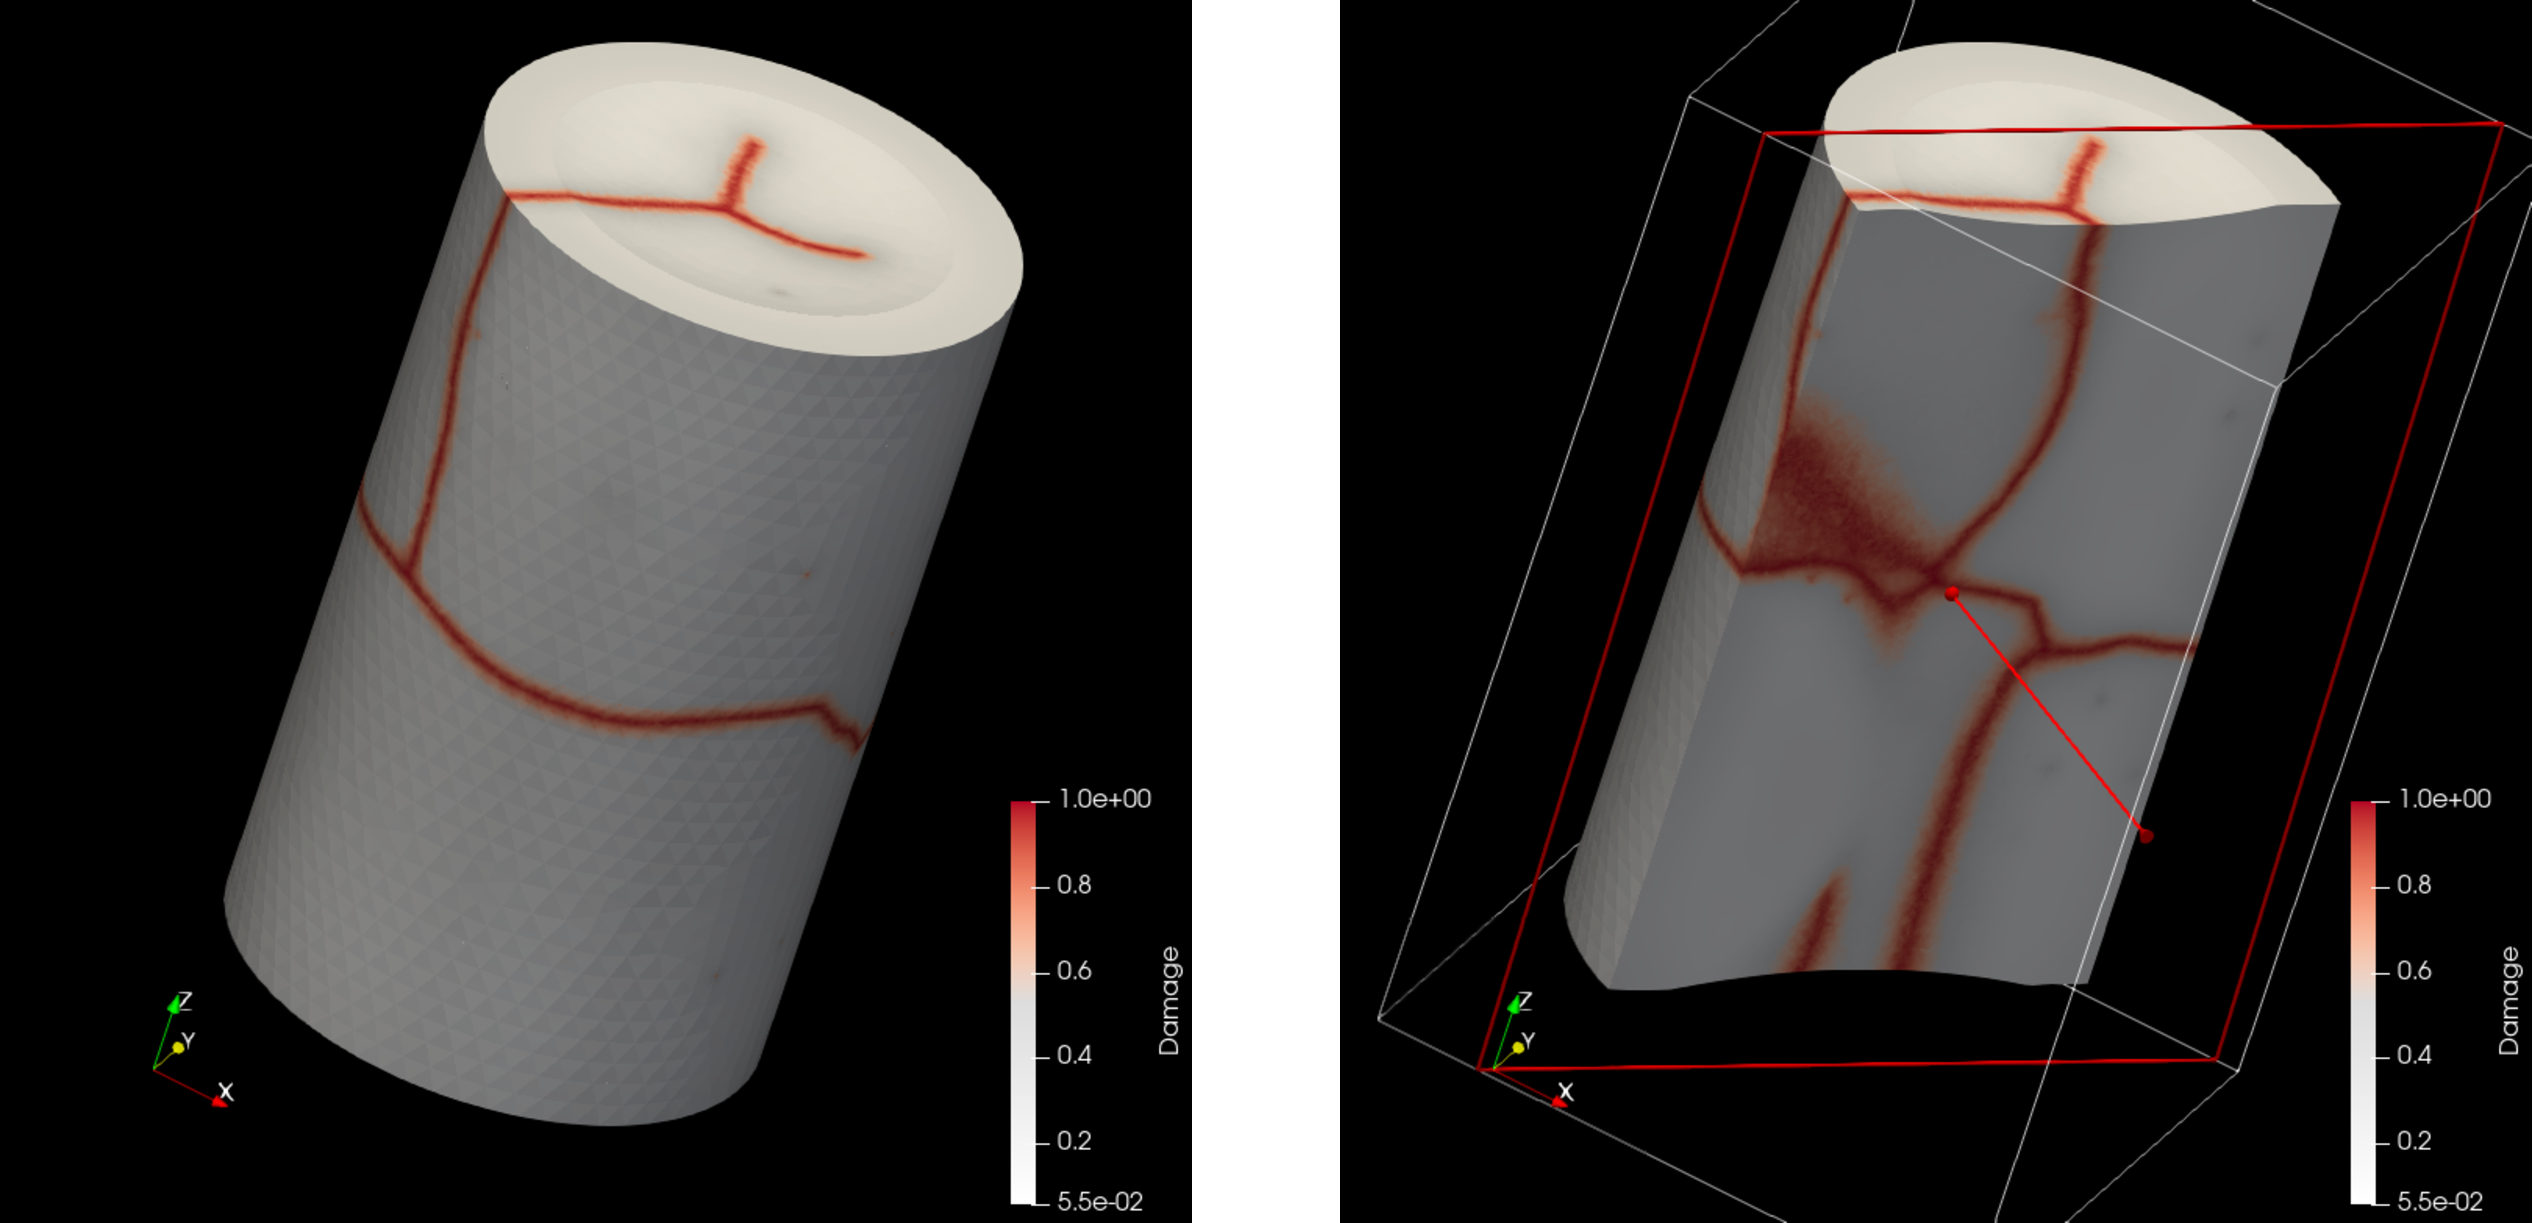
\includegraphics[width=14.cm]{../chapter_003_ef_micromorphic/figures/FuelPelletCracking-results.pdf}
  \caption{Crack pattern}
  \label{fig:micromorphic_damage:pellet_cracked}
\end{figure}